\documentclass[a4paper, 10pt]{article}

\usepackage[utf8]{inputenc}
\usepackage[spanish]{babel}
\usepackage{graphicx}
\usepackage{geometry}
\usepackage{listings}
\usepackage{amsmath}
\usepackage{amsfonts}
\usepackage{amssymb}
\usepackage{caratula}
\usepackage[section]{placeins}
\usepackage{titlesec}

\newcommand{\Z}{\mathbb{Z}}
\def\code#1{\texttt{#1}}
\newcommand\tab[1][0.5cm]{\hspace*{#1}}

\geometry{a4paper, margin=0.7in}

\begin{document}
    %Caratula
    \pagenumbering{gobble}
    \newpage

    \begin{center}
        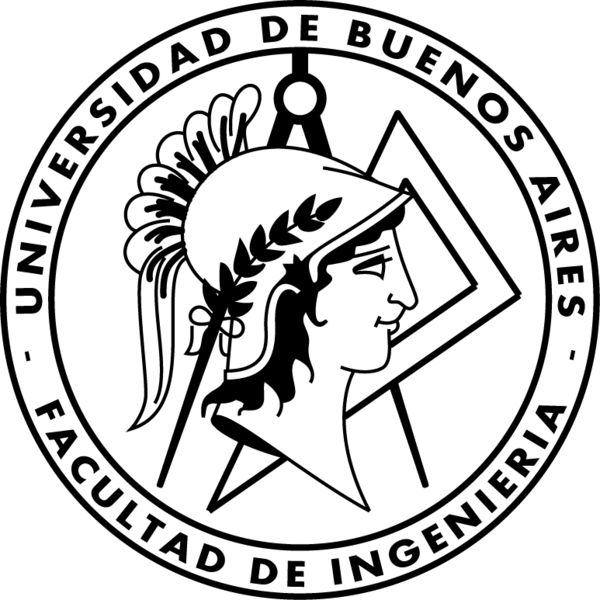
\includegraphics[width=7.5cm, height=7.5cm]{images/logo}
    \end{center}

    \materia{Organización de Datos}
    \submateria{Segundo Cuatrimestre 2017}
    \titulo{Trabajo Práctico 1}

    \integrante{Rodrigo De Rosa}{97799}{rodrigoderosa@outlook.com}
    \integrante{Marcos Schapira}{97934}{schapiramarcos@gmail.com}
    \integrante{Facundo Guerrero}{97981}{facundoiguerrero@gmail.com}
    \maketitle
    %Fin caratula
    %Table of contents
    \newpage
    \pagenumbering{roman}
    \tableofcontents
    %Fin table of contents
    %Informe
    \newpage
	\pagenumbering{arabic}
	\part{Análisis del precio por $m^2$}
		\section{Adaptación del DataFrame}
			Para el análisis particular de cada característica de la información que se posee, se adaptó el DataFrame
			original para poder analizar dicha información mas fácil y comodamente.
			\subsection{Filtrado de columnas}
				Para el análisis de esta cierta característica de las propiedades, consideramos \emph{importantes}
				sólo a algunas celdas. Estas son:
				\begin{itemize}
					\item \code{place name} $\leftarrow$ \code{location}
					\item \code{price aprox usd} $\leftarrow$ \code{price}
					\item \code{surface total in m2} $\leftarrow$ \code{totalSurface}
					\item \code{surface covered in m2} $\leftarrow$ \code{coveredSurface}
					\item \code{price usd per m2} $\leftarrow$ \code{pricem2}		
				\end{itemize}
			\subsection{Completando el DataFrame}
				Lo primero que se hizo para realizar este analisis fue completar las columnas faltantes
				de la mayor cantidad de entradas posibles. Esto es, \code{location, price, totalSurface,
				pricem2}. De esta forma, nos permitimos analizar una mayor cantidad de propiedades
				para realizar un analisis un poco mas correcto. \\
				\tab Para completar el campo de precio por $m^2$ se necesita que la entrada sobre la que
				se trabaja cumpla la siguiente condición lógica: $price_{}m^2 \vee (price \wedge surface)$. Es
				decir, necesita tener o el precio por metro cuadrado o tanto el precio total como la superficie
				total. \\
				\tab Si el campo \code{pricem2} tiene valor, entonces ese será el utilizado. En caso contrario,
				si tanto el campo \code{price} como el campo \code{totalSurface} tienen valor, definimos como
				nuestro nuevo \code{pricem2} a la división $\frac{price}{surface}$. \\
				\tab Para esto, necesitamos unificar \code{coveredSurface} y \code{totalSurface}, para maximizar
				nuevamente la cantidad de entradas disponibles. Esto se hace, simplemente, poniendo como
				\code{totalSurface} el valor de \code{coveredSurface} en aquellas entradas donde la primera
				no tenga valor (consideramos que $total - covered = uncovered$). \\
				\tab Una vez completados todos los \code{pricem2} posibles, eliminamos todas aquellas entradas
				que tengan \code{NaN} como valor (en cualquiera de las celdas que definimos como \emph{importantes}),
				pues ya no podemos obtener el valor de esa celda de ningun otro lugar.
		\section{Estudio estadístico de los datos}
			\subsection{Analisis de la distribución de precios}
				Una vez completado el DataFrame lo mas posible, se realizó un análisis de la distribución de precios.
				Con esto nos referimos a analizar la variación del precio por metro cuadrado entre todas las
				propiedades. Es decir, \emph{limpiar los datos que no tienen sentido}. \\
				\tab Para esto le pedimos el \code{.describe()} a nuesto DataFrame con los percentiles $0.01$ y
				$0.99$. Esto nos permite analizar que tan desviados estan los valores máximos y mínimos. \\
				\tab Con los percentiles recién mencionados hacemos un recorte de los datos para lograr una distribución
				que se asemeje a una Normal lo mas posible. El primer recorte es tanto inferior ($ > 150$USD) como superior
				($<18000$USD). Como en este nuevo DataFrame la diferencia entre el percentil $0.99$ y el máximo es de más
				del doble, se vuelve a recortar superiormente ($<8000$USD). \\
				\tab Luego de esto, la distribución de precios es un poco mejor que antes (las diferencias entre los
				percentiles $0.25, 0.5, 0.75$ son similares). \\
				\tab A continuación se muestra un gráfico de distribución de precios por metro cuadrado que se obtiene
				del DataFrame original sin realizar el filtrado recién mencionado. Nos hubiese gustado poder mostrar tanto
				el KDE como el histograma pero al haber tanta diferencia entre el maximo y los valores principales de la
				distribución, el histograma era solo una linea. El objetivo de este gráfico es hacer incapié en lo mencionado
				en el previo párrafo: es necesario filtrar los datos para tener un conjunto de datos con sentido.
				\begin{center}
       				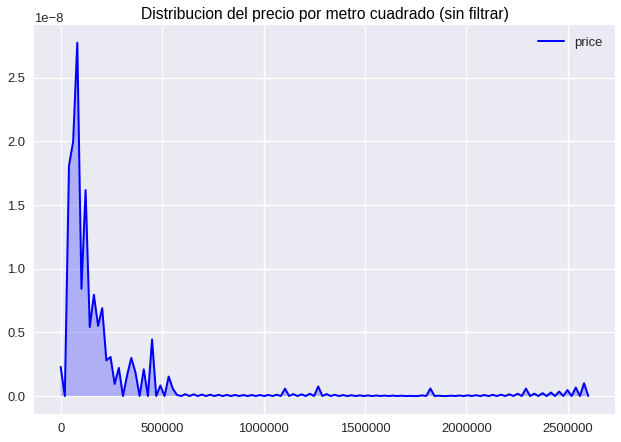
\includegraphics[width=\textwidth]{images/m2UnfilteredKDE}
		   		\end{center}
				\tab En el siguiente gráfico de distribución de precios por metro cuadrado se puede ver que la mayor parte
				de las propiedades están concentradas en el rango de precios $[150;4000]$USD y luego hay un drástico decaimiento
				de cantidad de propiedades para el resto de los precios. Si bien se podría considerar que un recorte sería
				correcto, a partir de fuentes externas se sabe que ciertos barrios (\emph{i.e.} Puerto Madero) tienen,
				aproximadamente, un valor medio de $6000$USD por metro cuadrado.
				\begin{center}
       				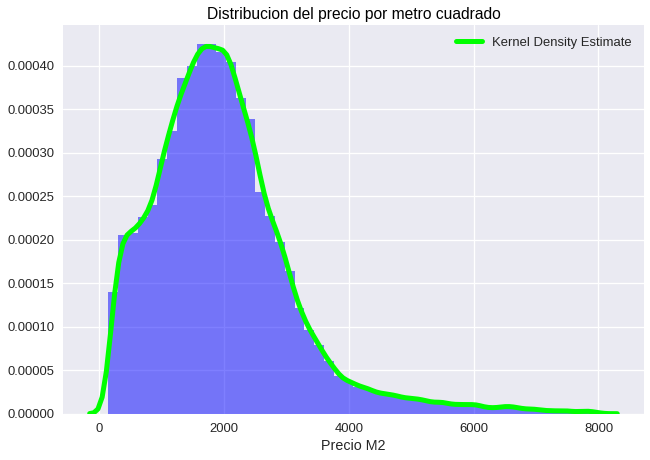
\includegraphics[width=\textwidth]{images/m2Histogram}
		   		\end{center}
			\subsection{Agrupando por barrios}
				Ahora que nuestros datos están tan completos y retocados como querríamos, procedemos a agrupar todas las propiedades
				de acuerdo al barrio al que pertencen. Una vez que los tenemos agrupados, debemos establecer un \emph{minimo de
				propiedades} por barrio. Pues un barrio que tiene una o dos propiedades podría alterar el estudio de la
				informacion. \\
				\tab Nuevamente, para esta tarea utilizizamos \code{.describe()} y resolvemos que utilizaremos como cota inferior
				$50$ propiedades (dos mas que el equivalente a una publicación por mes en los últimos cuatro años). \\
				\tab Aquí, al igual que hicimos antes, mostraremos la distribución antes y después del filtro aplicado. Si bien
				en escencia no son tan diferentes, podemos observar que desaparecen algunos barrios de la zona de precios altos.
				\begin{center}
       				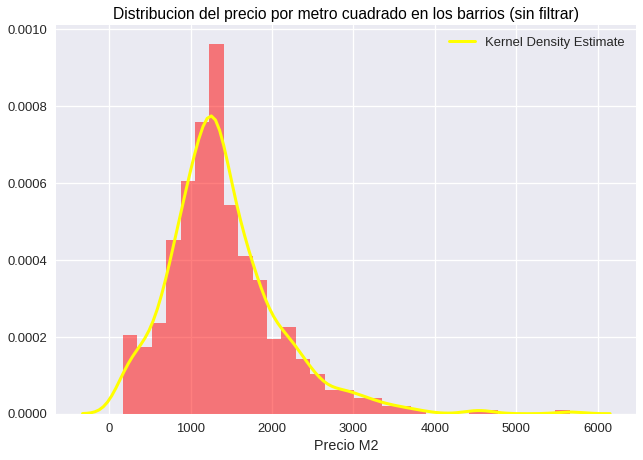
\includegraphics[width=\textwidth]{images/m2HoodUnfilteredKDE}
		   		\end{center}
				\tab Una vez que eliminamos los barrios problemáticos, si analizamos la distribución de precio por barrio
				podemos ver que la mayor parte está concentrada en el intervalo $[500;3500]$USD, mientras que muy pocos
				(solo tres) superan ese valor.
				\begin{center}
   	    				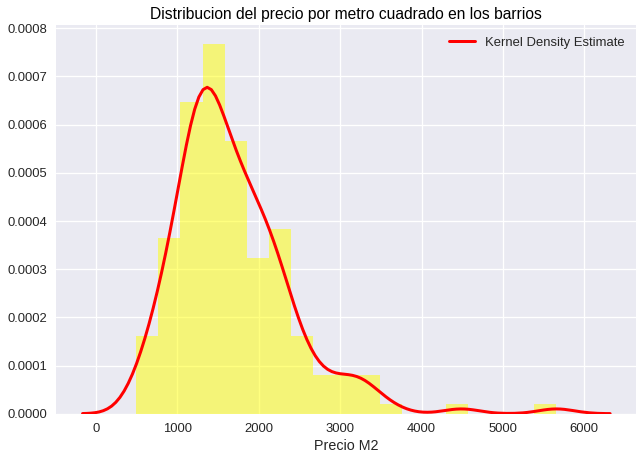
\includegraphics[width=\textwidth]{images/m2HoodHistogram}
			    \end{center}	
			    \tab Podemos ver, además, que la distribución es bastante similar a la anterior (sin agrupar por barrios) aunque,
			    obviamente, con valores menores (pues son promedios).
		\section{Analizando grupos característicos}
			En esta sección analizaremos ciertos grupos característicos a partir de la información con la que estamos trabajando.
			\subsection{Los diez barrios con mayor precio por $m^2$}
				Dado que ya estamos felices con la forma en que tenemos dispuestos los datos, comenzaremos por hacer un
				\emph{Top 10} de los barrios más caros de CABA y GBA. \\
				\tab Para esto, como ya tenemos los datos agrupados, simplemente ordenamos el DataFrame y nos quedamos con
				los primeros diez.
				\tab Durante el análisis de esta información, notamos que varios de los barrios que aparecían en este \emph{Top 10}
				eran subdivisiones del barrio de Palermo. Por esta razón, decidimos incluir dos casos: uno en que consideramos
				que todos los 'Palermos' son uno solo, y otro en que cada uno es considerado un barrio diferente.
				\subsubsection{Unificación de Palermo}
					En este caso, consideramos que todas las subdivisiones de Palermo pertenecen a un sólo barrio.\\
					\tab El resultado obtenido es el siguiente:
					\begin{center}
						\begin{tabular}{ |c|c|c| }
							\hline
							\multicolumn{3}{|c|}{Top 10 [Palermo unificado]}\\
							\hline
							\hline
							Puesto & Barrio & Precio $m^2$ [U$\$$D] \\
							\hline
							1 & Puerto Madero & 5657 \\
							2 & Las Cañitas & 3612 \\
							3 & Palermo & 3518 \\
							4 & Recoleta & 3316 \\
							5 & Belgrano & 3124 \\
							6 & Nuñez & 3056 \\
							7 & Barrio Norte & 2949 \\
							8 & Vicente López & 2925 \\
							9 & Retiro & 2783 \\
							10 & Olivos & 2737 \\
							\hline
						\end{tabular}
					\end{center}
					\tab En la tabla se observa que Puerto Madero tiene un valor mucho mas alto que el resto, de hecho, es
					mayor al doble del precio del décimo. De todos modos, entre el segundo y el último la variación es más
					suave. Para aportar a este análisis, se realiza un gráfico de barras:
					\begin{center}
   	    					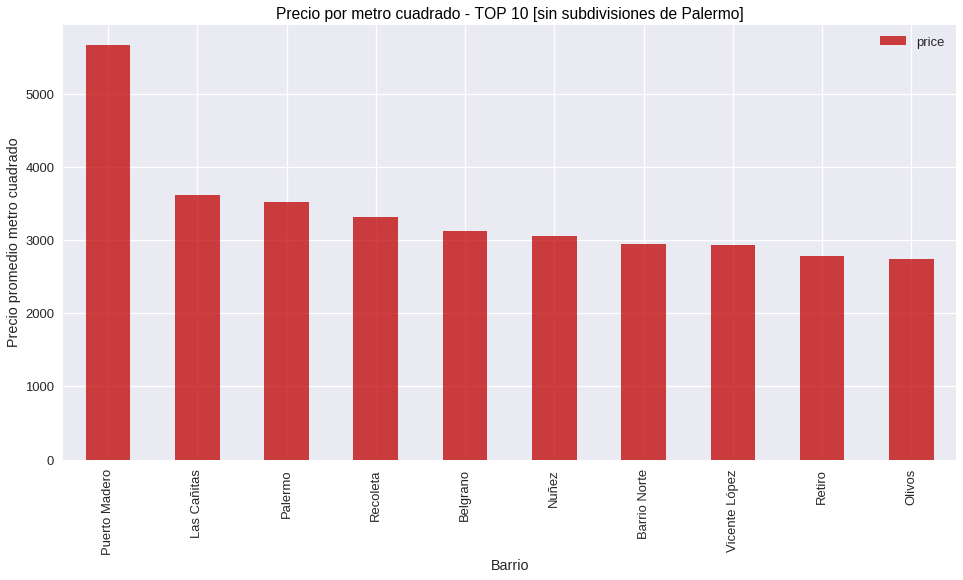
\includegraphics[width=\textwidth]{images/m2UnifiedTop10}
			  		\end{center}	
			  	\subsubsection{División de Palermo}
			  		Aquí consideraremos que el barrio al que se nombra Palermo corresponde a todas las secciones de dicho
			  		barrio que no son las que ya aparecen en otro grupo. \\
			  		\tab En este caso, el resultado obtenido es:
			  		\begin{center}
						\begin{tabular}{ |c|c|c| }
							\hline
							\multicolumn{3}{|c|}{Top 10 [Palermo dividido]}\\
							\hline
							\hline
							Puesto & Barrio & Precio $m^2$ [U$\$$D] \\
							\hline
							1 & Puerto Madero & 5657 \\
							2 & Palermo Chico & 4489 \\
							3 & Las Cañitas & 3612  \\
							4 & Palermo Viejo & 3419 \\
							5 & Recoleta & 3316 \\
							6 & Palermo & 3260 \\
							7 & Palermo Hollywood & 3224 \\
							8 & Palermo Soho & 3198 \\
							9 & Belgrano & 3124 \\
							10 & Nuñez & 3056 \\
							\hline
						\end{tabular}
					\end{center}
					\tab En la tabla podemos ver que, si bien es correcto y es un \emph{Top 10}, esta plagado de subdivisiones
					de Palermo y no nos permite tener un plano más general. \\
					\tab Aquí el gráfico de barras es muy similar aunque aparece Palermo Chico, que se acerca un poco mas
					al valor de Puerto Madero. De todos modos, la diferencia entre el primero y el segundo es muy grande
					como también lo es entre el segundo y el tercero, dejando la relación entre los valores igual de 'no suave'.
					\begin{center}
   	    					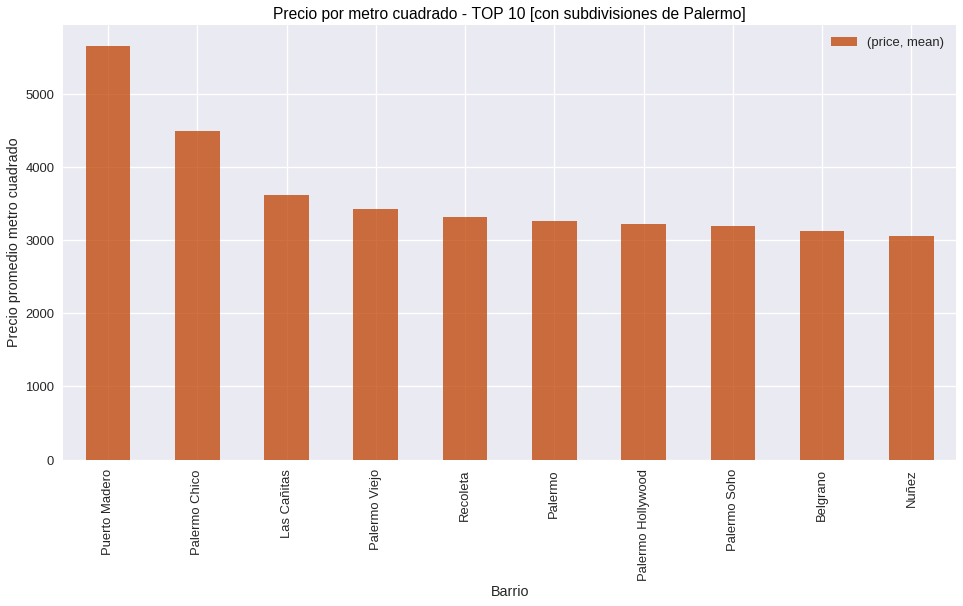
\includegraphics[width=\textwidth]{images/m2NotUnifiedTop10}
			  		\end{center}
			  		\tab De aquí en más, utilizaremos a Palermo como un barrio unificado.
			  	\subsubsection{Comentario sobre el Top 10}
				  	Este \emph{Top 10} arroja los resultados que se hubieran esperado, pues los únicos dos valores que no pertenecen
			  	a CABA corresponden a los primeros dos barrios de GBA en los que se piensa al pensar en los barrios mas caros
			  	de Buenos Aires. \\
			  		\tab Por otro lado, si nos sorprende el hecho de que el $m^2$ en Barrio Norte sea más barato que Núñez o en
			  		Belgrano.
			\subsection{Los diez barrios con menor precio por $m^2$}
				Para esta parte, al igual que antes, ordenamos los datos para analizar cuales son los diez barrios que se encuentran
				en el \emph{Bottom 10}. \\
				\tab Al realizar este análisis, lo obtenido es:
				\begin{center}
					\begin{tabular}{ |c|c|c| }
						\hline
						\multicolumn{3}{|c|}{Bottom 10}\\
						\hline
						\hline
						Puesto & Barrio & Precio $m^2$ [U$\$$D] \\
						\hline
						1 & Ingeniero Pablo Nogués & 494 \\
						2 & Maschwitz & 548 \\
						3 & Villa Udaondo & 558 \\
						4 & Parque Leloir & 579 \\
						5 & Presidente Perón & 643 \\
						6 & Benavidez & 705 \\
						7 & José C Paz & 711 \\
						8 & Villa Libertad & 743 \\
						9 & Longchamps & 800 \\
						10 & Burzaco & 804 \\
						\hline
					\end{tabular}
				\end{center}
				\tab Si graficamos estos valores al igual que antes podremos ver un ascenso (o descenso) más suave que el del
				\emph{Top 10}. Si bien el primero es casi la mitad de el último, la variación entre puestos es menor. \\
				\begin{center}
   	    				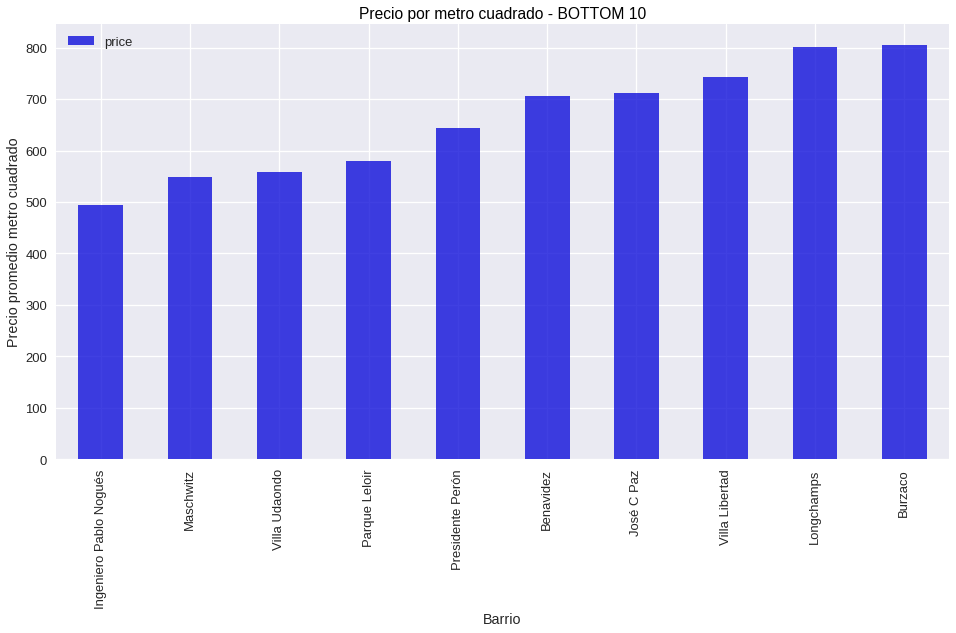
\includegraphics[width=\textwidth]{images/m2Bottom10}
			  	\end{center}
				\tab Aquí, remitiéndonos a la sección 3.1.3, vemos que los barrios del \emph{Bottom 10} son todos barrios
				alejados de la ciudad, de los cuales es esperable un bajo valor del $m^2$.
			\subsection{Dividiendo en secciones}
				El objetivo de esta parte es determinar diferentes grupos de barrios basados en el precio promedio del $m^2$
				para, de esta manera, analizar que tan suave (o no) es el decrecimiento del valor del $m^2$ en cada uno de
				estos grupos. \\
				\tab Los barrios serán divididos en grupos a partir de valores arbitrarios de precio por $m^2$, que surgen de
				un análisis de los datos. Los grupos serán:
				\begin{center}
					\begin{tabular}{ |c|c|c| }
						\hline
						\multicolumn{3}{|c|}{Divisones} \\
						\hline
						\hline
						Numero & min(price$m^2$) [USD] & max(price$m^2$) [USD] \\
						\hline
						1 & $2500$ & $\infty$ \\
						\hline
						2 & $2000$ & $2499$ \\
						\hline
						3 & $1500$ & $1999$ \\	
						\hline
						4 & $1200$ & $1499$ \\
						\hline
						5 & $950$ & $1199$ \\		
						\hline
						6 & $450$ & $949$ \\			
						\hline
					\end{tabular}
				\end{center}
				\tab El siguiente gráfico de área muestra el precio del $m^2$ y las divisiones (diferentes intensidades de
				azul) indican los diferentes grupos.
				\begin{center}
   	    				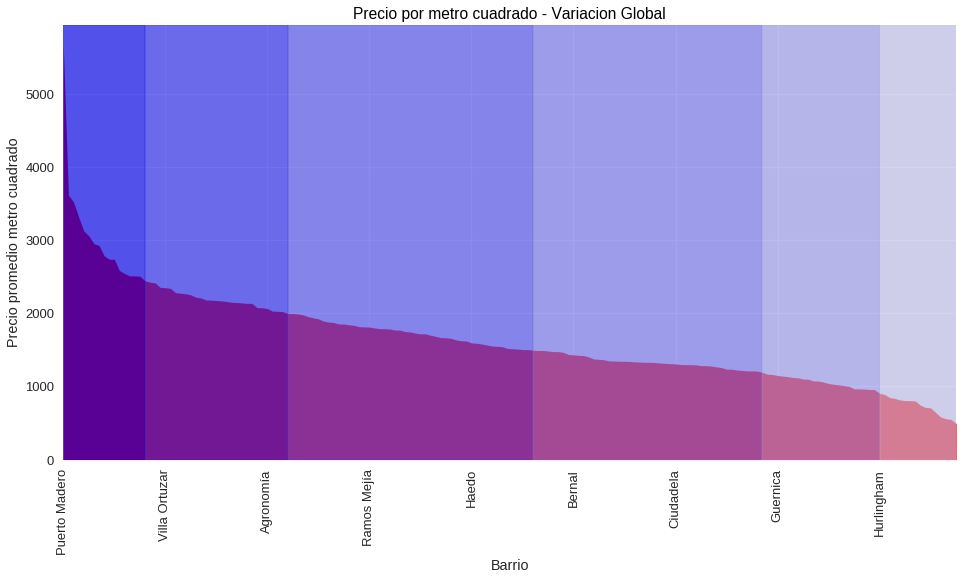
\includegraphics[width=\textwidth]{images/m2HoodsDivision}
			  	\end{center}
			  	\tab Nos interesa mostrar también que porcentaje de los barrios está incluído en cada uno de estos grupos para
			  	saber en cuál de ellos se concentra la mayor parte.
			  	\begin{center}
			  		\begin{tabular}{ |c|c|c| }
						\hline
						\multicolumn{3}{|c|}{Distribución en grupos} \\
						\hline
						\hline
						Grupo & Cantidad de barrios & Porcentaje \\
						\hline
						1 & 16 & $9\%$ \\
						\hline
						2 & 28 & $16\%$ \\
						\hline
						3 & 48 & $27\%$ \\
						\hline
						4 & 45 & $26\%$ \\
						\hline
						5 & 23 & $13\%$ \\
						\hline						
						6 & 16 & $9\%$ \\
						\hline						
			  		\end{tabular}
				\end{center}			  	 
				\tab Vemos que, como se puede apreciar en el gráfico, los grupos $3$ y $4$ son los que concentran a la mayor
				cantidad de barrios. De hecho, entre ellos dos tienen a más del $50\%$. \\
				\tab Ahora procedermos a analizar grupo por grupo.
				\subsubsection{Grupo 1 - $[2500:\infty)$U$\$$D}
					En este grupo se encuentra a los dieciséis barrios más caros de CABA y GBA. Aunque a los primeros diez ya los
					conocemos de la sección 3.1, lo que nos interesa en esta parte es analizar y comparar cómo varía el precio
					del metro cuadrado grupo a grupo mas que los nombres propios de cada integrante de cada grupo. En cada uno
					de los grupos se mostrará un \emph{zoom} del gráfico de área previo, para agregar una visualización al
					análisis de la variación en cada caso. \\
					\tab En este caso, lo que esperamos encontrar es un inicio con una pendiente muy inclinada y, a medida que
					nos alejamos del primer barrio (que ya sabemos que es Puerto Madero), un decrecimiento de dicha pendiente,
					pues la diferencia entre barrio y barrio será mucho menor, aunque seguirá siendo el grupo con mayor variación
					entre barrios de todos.
					\begin{center}
   		    				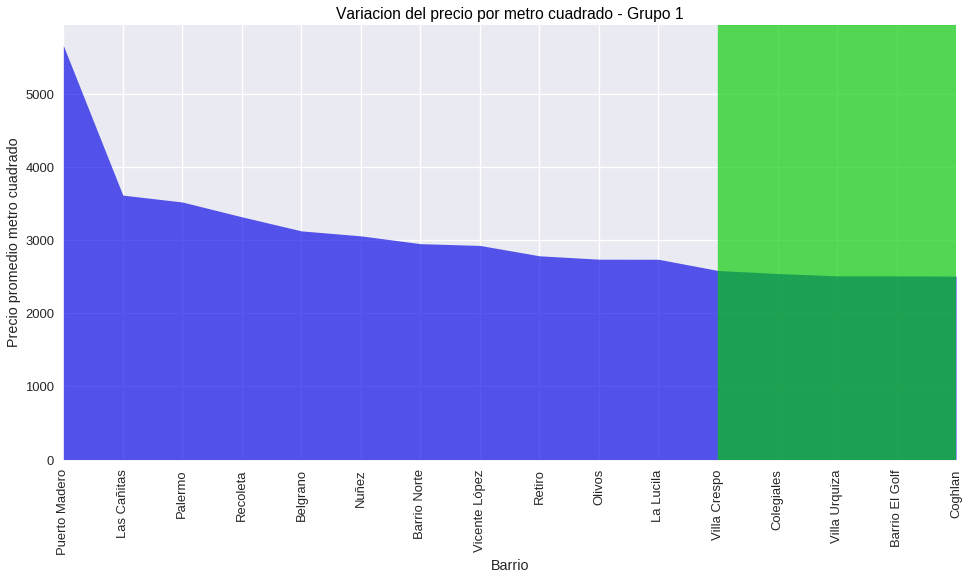
\includegraphics[width=\textwidth]{images/m2Group1Area}
				  	\end{center}
				  	\tab Si bien el gráfico muestra lo que se esperaba, también se ve que a partir del doceavo barrio la curva
				  	se vuelve casi constante (en verde), mostrando que hay un cierto subgrupo de barrios con precios muy 
				  	similares. Esto se puede ver en el gráfico de la sección anterior si se observa el pequeño valle que 
				  	se forma justo antes 	de llegar a la división entre el grupo 1 y el 2. \\
				  	\tab Cabe destacar, además, que si no fuera por el precio extraordinario de Puerto Madero, el grupo tendría
				  	una variación mucho menor, pues iría entre $3600$USD y $2500$USD lo que representaría una variación de
				  	$1100$USD ($30\%$) entre el máximo y el mínimo mientras que, actualmente, la variación es de $3100$USD
				  	($55\%$).
				\subsubsection{Grupo 2 - $[2000:2500)$U$\$$D}
					Observando el gráfico en el que se realizaron las divisiones por grupo esperamos que este segundo grupo
					tenga un sector medio con pendiente casi nula, donde la diferencia entre el precio en un barrio y el
					siguiente sea casi nula.
					\begin{center}
   		    				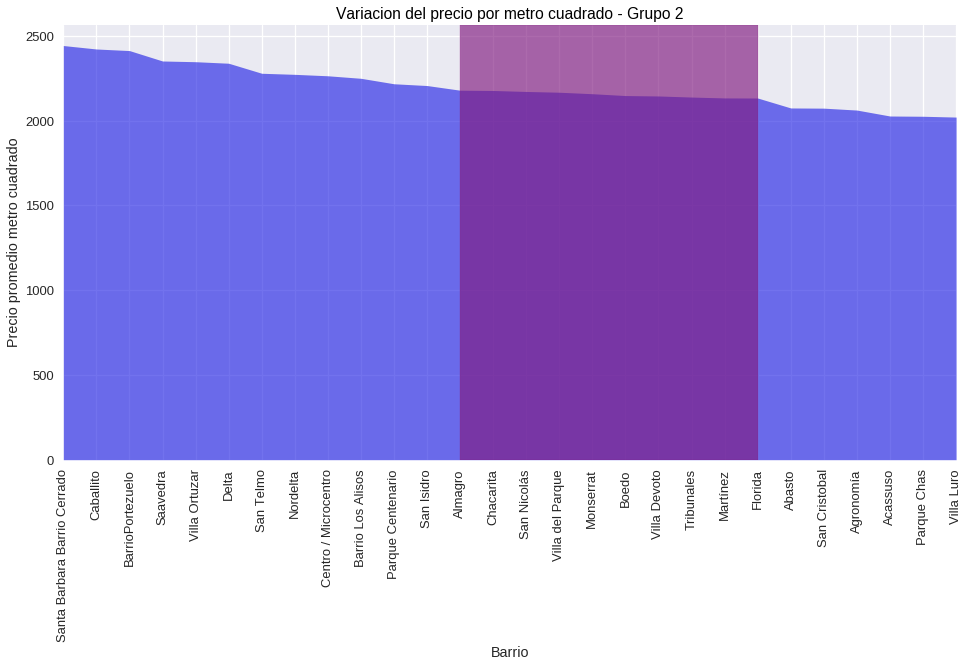
\includegraphics[width=\textwidth]{images/m2Group2Area}
				  	\end{center}
				  	\tab El sector indicado el violeta es aquel que mencionamos previamente con pendiente casi nula. En este
				  	subgrupo se encuentran diez barrios y la diferencia entre el primero y el último es de solamente $46$USD.
				  	Dado los numeros que se manejan, esa diferencia es casi despreciable, teniendo así un subgrupo de diez 
				  	barrios con el mismo valor para el $m^2$. \\
				  	\tab En cuanto al porcentaje de variación, a partir de este segundo grupo lo podemos dividir en dos; uno
				  	particular del grupo, en donde el porcentaje se calcula a partir del máximo local, y otro general, en donde
				  	el porcentaje se calcula a partir del máximo global (\emph{i.e.} Puerto Madero). La diferencia entre el
				  	máximo local y el mínimo es de $422$USD, siendo, de esta manera, la variación local del $17\%$ y la general
				  	del $7\%$. \\
				  	\tab Vemos entonces que la diferencia de variación ya decreció en gran medida pasando del grupo 1 al grupo 2.
				\subsubsection{Grupo 3 - $[1500:2000)$U$\$$D}
					Ahora llegamos al primero de los dos grupos principales. Como vimos antes, este grupo concentra al $27\%$ de
					los barrios de CABA y GBA pero (según nos muestra a grandes rasgos el gráfico general) con mayor variación
					que el próximo grupo, que también concentra a una gran parte de los barrios.\\
					\tab En este caso, esperamos ver una pendiente casi constante en todo el grupo sin regiones con pendiente
					casi nula pero con una variación pequeña entre un barrio y el siguiente.
					\begin{center}
   		    				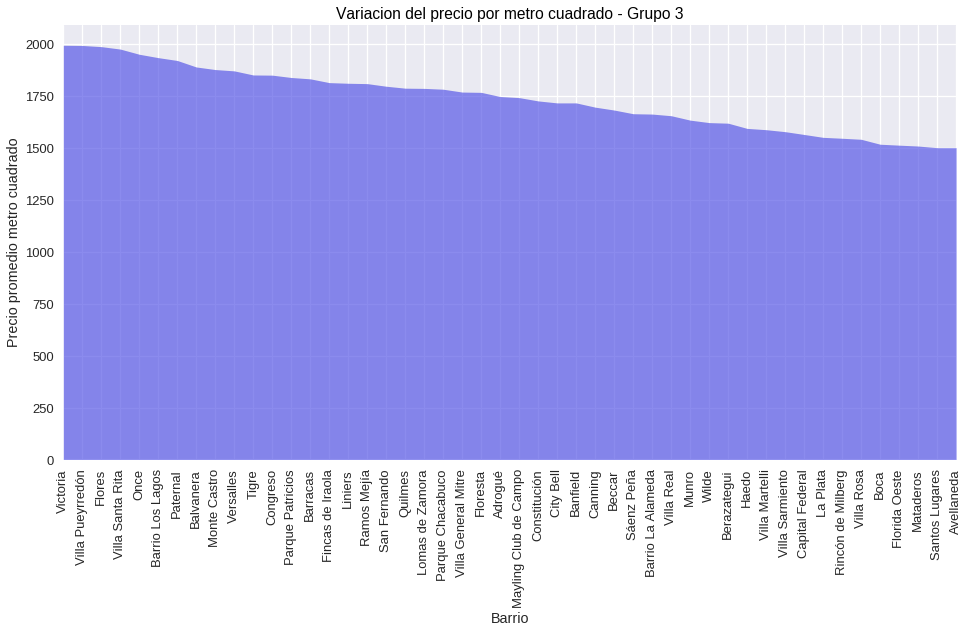
\includegraphics[width=\textwidth]{images/m2Group3Area}
				  	\end{center}
				  	\tab En este gráfico se observa lo previamente indicado, el decrecimiento es bastante lineal y no se detectan
				  	zonas con precios constantes. De todas formas, si se amplía un poco, se pueden encontrar pares o tríos de grupos
				  	que tienen precios similares, como se ve a continuación.
				  	\begin{center}
   		    				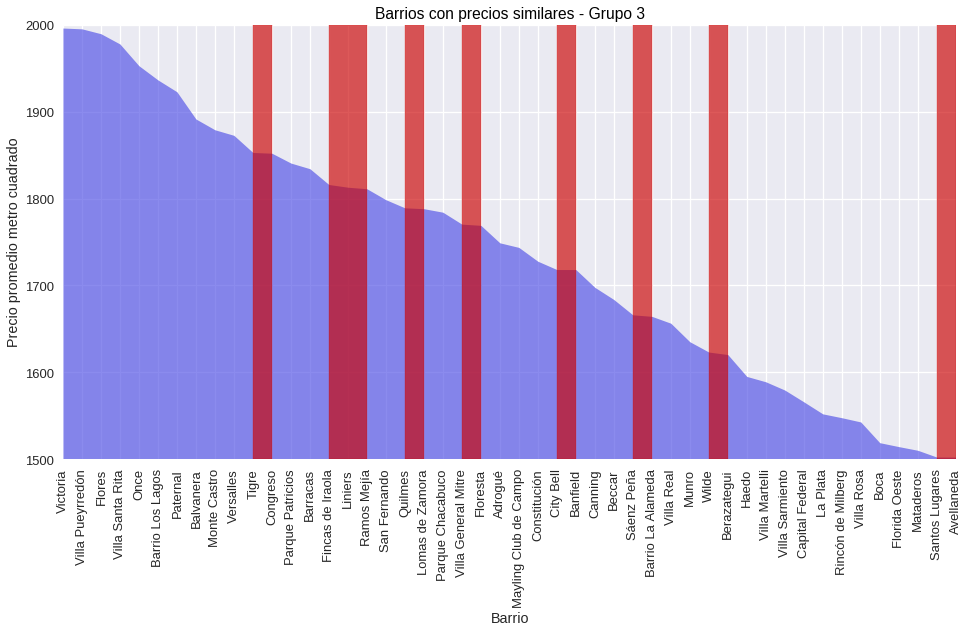
\includegraphics[width=\textwidth]{images/m2Group3Detail}
				  	\end{center}
				  	\tab Aquí podemos ver que si bien hay diecisiete barrios que comparten precio con algún otro, no son contiguos
				  	como en el grupo 2. De todas maneras, como en este grupo la variación general de precio es menor y la cantidad
				  	de barrios es mayor, podríamos encontrar también un grupo de diez barrios con variación de aproximadamente
				  	$50$USD. Por ejemplo, entre Monte Castro y Ramos Mejía hay una diferencia de $60$USD y se encierra un subgrupo
				  	de nueve barrios. \\
				  	\tab Analizando el porcentaje de variación al igual que en el Grupo 2, sabiendo que la diferencia entre el
				  	máximo local y el mínimo es de $493$USD, el porcentaje de variación local es de un $25\%$ y el porcentaje
				  	de variación global es del $9\%$. \\
				  	\tab Se observa entonces que, lógicamente, ahora que estamos en una zona de precios menores, una diferencia
				  	entre mínimo y máximo similar a la del grupo anterior ahora representa una variación mayor. Por otro lado,
				  	la variación global es apenas mayor a la del grupo anterior. De todas formas, estos porcentajes están sujetos
				  	a la división arbitraria de los grupos hecha previamente (pues el máximo delta es $500$USD).
				\subsubsection{Grupo 4 - $[1200:1500)$U$\$$D}
					Este cuarto grupo es el segundo grupo principal, concentra el $26\%$ de todos los barrios y es el de menor
					rango de valores, con $300$USD, salvo por el grupo 5, con $250$USD. Esto nos dice que la pendiente en este
					caso será la menor de todas, como se puede ver en el gráfico general. Además, esperamos ver una zona central
					con pendiente casi nula, en donde se encontrará un grupo muy grande de barrios con una variación en el precio
					muy pequeña, a diferencia del grupo 3.
					\begin{center}
   		    				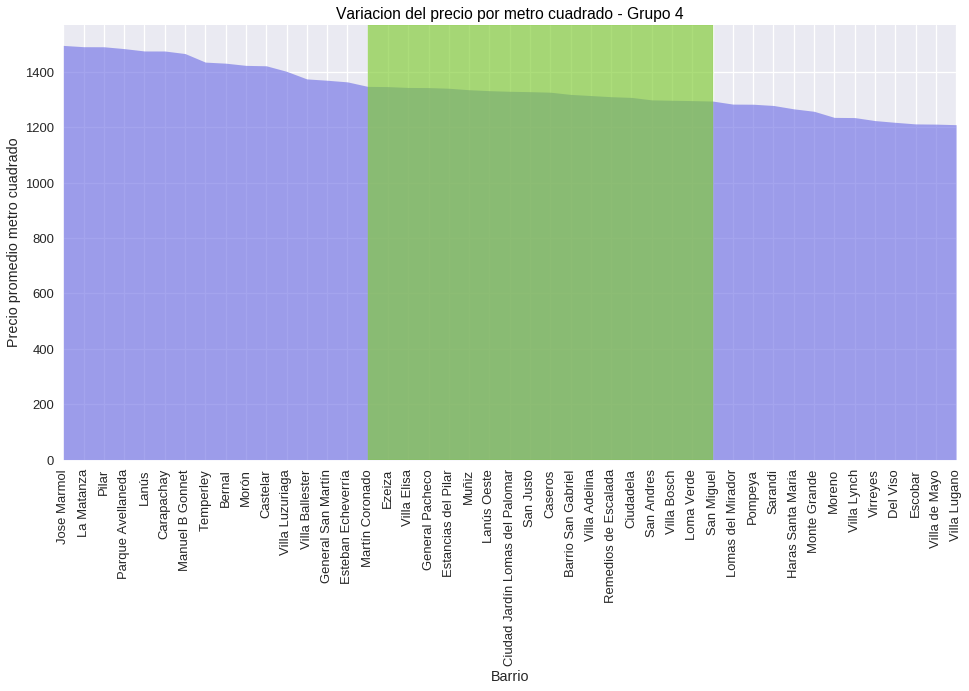
\includegraphics[width=\textwidth]{images/m2Group4Area}
				  	\end{center}
				  	\tab El subgrupo indicado con verde consiste de dieciocho barrios que se diferencian solamente, entre el primero
				  	y el último, por $53$USD. Como supusimos, en este grupo se encuentra el conjunto de barrios con variación casi
				  	nula más grande de todos. Adicionalmente, si se observa el gráfico con atención, en la mayor parte se encuentran
				  	subgrupos pequeños con valores casi constantes hasta que hay un pequeño descenso de precio, nuevamente un valor
				  	casi constante, etc. dividiendo el grupo en cinco o seis diferentes subgrupos pequeños (o no tanto, como el
				  	verde) por lo que no tiene sentido destacarlos como en el grupo 3, pues solo quedarían aquellos pequeños sectores
				  	donde la pendiente si toma valor considerable. \\
				  	\tab En cuanto al porcentaje de variación, sabiendo que la diferencia entre el máximo local y el mínimo es de
				  	$286$USD, tenemos un porcentaje de variación local del $19\%$ y uno global del $5\%$. Por lo tanto, y como era
				  	de esperarse, este grupo tiene los porcentajes mínimos en ambos casos; en el local porque tiene la mayor cantidad
				  	de segmentos casi constantes y en el global porque, además de la razón recién mencionada, por tener valores
				  	cada vez más bajos. Cabe destacar, además, que el $19\%$ local está concentrado en ciertos 'saltos' de un
				  	barrio a otro; pues, como mencionamos antes, la mayor parte del grupo esta compuesta por subgrupos de precios
				  	similares.
				\subsubsection{Grupo 5 - $[950:1200)$U$\$$D}
					Este quinto y penúltimo grupo comienza una pendiente que incrementa progresivamente hacia el último y sexto
					grupo. Aquí se concentra el $13\%$ de los barrios, la mitad que en el grupo anterior, y los precios de los
					barrios ya se acercan a los minimos que se pueden encontrar.\\
					\tab A partir de la información que brinda el gráfico general, esperamos encontrar una pequeña zona de pendiente
					casi nula hacia el final del grupo y una variación local relativamente chica.
					\begin{center}
   		    				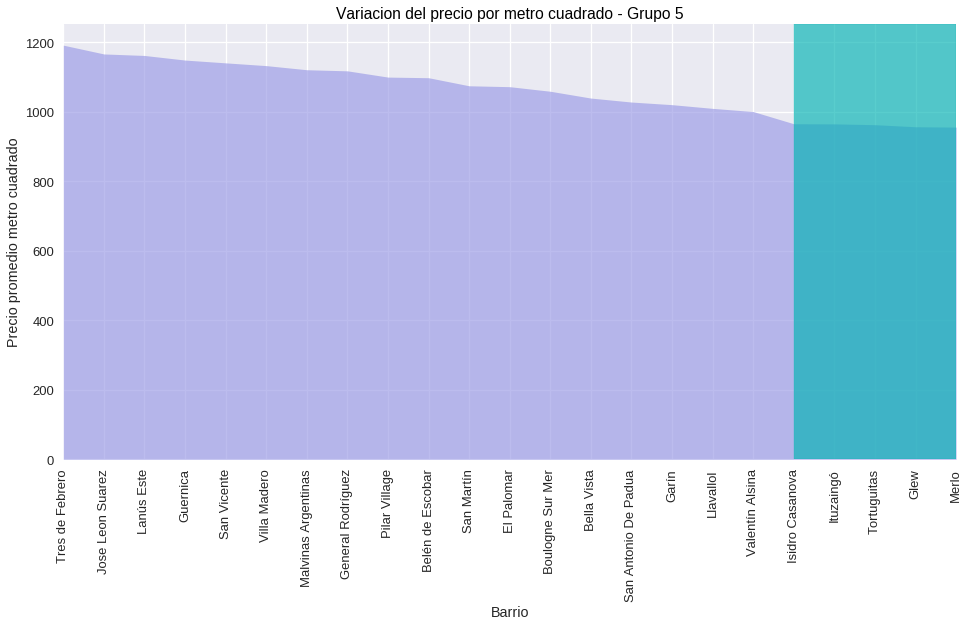
\includegraphics[width=\textwidth]{images/m2Group5Area}
				  	\end{center}
				  	\tab Indicado con color Cyan en el gráfico podemos ver ese pequeño grupo del que hablábamos donde la pendiente
				  	es casi nula, mientras que en el resto del grupo hay una pendiente casi constante. El tamaño de este subgrupo
				  	es de cinco barrios y la diferencia de precio entre el primero y el último es de $11$USD. \\
				  	\tab Si calculamos el porcentaje de variación, conociendo que la diferencia entre el máximo local y el mínimo
				  	es de $235$USD, obtenemos un porcentaje de variación local del $20\%$ y uno global del $4\%$. En este caso, el
				  	porcentaje local esta distribuido a lo largo de todo el grupo, salvo por el subgrupo final que tiene un valor
				  	casi constante.
				\subsubsection{Grupo 6 - $[450:950)$U$\$$D}
					En este último grupo, que contiene sólo al $9\%$ de los barrios (al igual que el grupo 1), estaremos analizando
					a aquellos barrios con menor precio por $m^2$. A partir del gráfico general sabemos que la pendiente será muy
					marcada y que la diferencia entre un barrio y el siguiente será importante, salvo por una pequeña parte donde
					los precios se mantendrán casi constantes.
					\begin{center}
   		    				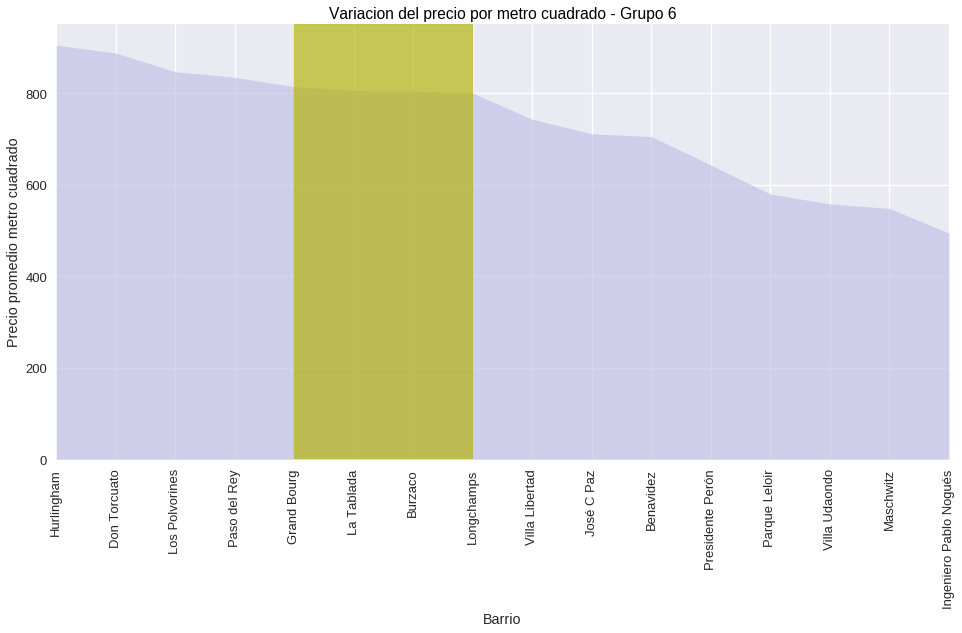
\includegraphics[width=\textwidth]{images/m2Group6Area}
				  	\end{center}
					\tab En amarillo se puede observar la única sección casi constante del grupo, que consta sólo de cuatro barrios
					y que contienen un rango cuya diferencia entre el mínimo y el máximo es de $14$USD. Mientras tanto, el resto
					del grupo tiene una pendiente considerablemente grande y la diferencia entre el valor máximo y el mínimo es casi
					del doble. \\
					\tab Para remarcar esto último, calcularemos el porcentaje de variación sabiendo que dicha diferencia es de
					$410$USD. El porcentaje de variación local es del $45\%$ y el porcentaje de variación global es del $7\%$. Aquí
					la variación local está repartida en todo el grupo pero con mayor participación de la segunda mitad, donde la
					pendiente es mayor, y con menor participación del sector casi constante.\\
		\section{Distribución geográfica}
			En esta sección se mostrará, con la ayuda de \emph{HeatMaps} cómo están distribuídos los precios por $m^2$ en CABA
			y GBA. \\
			\tab Para empezar, mostraremos un mapa general de CABA y GBA donde la unidad de medida es el precio por $m^2$. Se
			debe tener en cuenta que el software utilizado determina el color de un pixel a partir de la suma de todas las
			propiedades que se corresponden con ese pixel, y por dicha razón, podríamos encontrar sectores donde, si bien el
			precio no es tan elevado, hay muchas propiedades y por ende se las indica con rojo. De todas formas, este gráfico
			nos sirve para tener un plano general.
			\begin{center}
				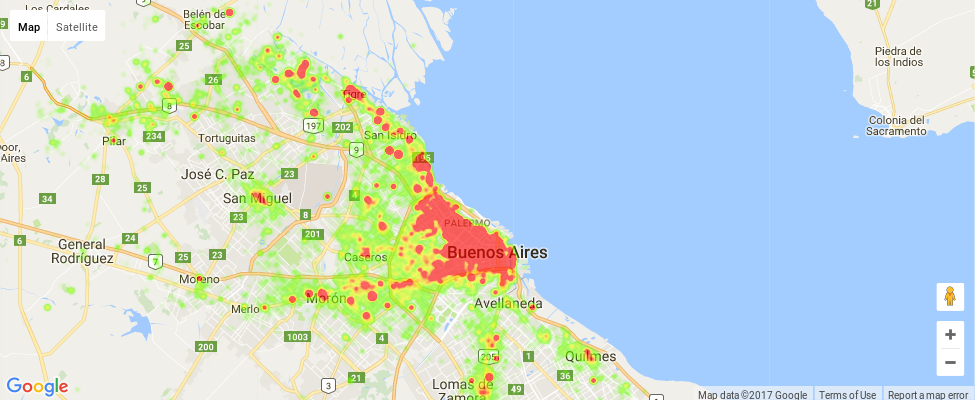
\includegraphics[width=\textwidth]{images/m2GeneralHeatMap}
		  	\end{center}
			\subsection{Grupos característicos y su ubicación}			
				Ahora, lo que haremos será repetir la dinámica pero dividiendo en los mismo grupos característicos de antes, para
				ver que se puede saber de cada grupo según su ubicación. Cabe destacar que la escala de precios utilizada en los
				mapas de cada grupo es diferente, pues el objetivo aquí es mostrar la ubicación de estos barrios más que el valor
				que ellos tienen.
				\subsubsection{Grupo 1}
					Para el grupo 1, como se dijo previamente, se espera encontrar a las propiedades en CABA y la zona de GBA
					que corresponde al inmediato Norte de la Capital Federal.
					\begin{center}
						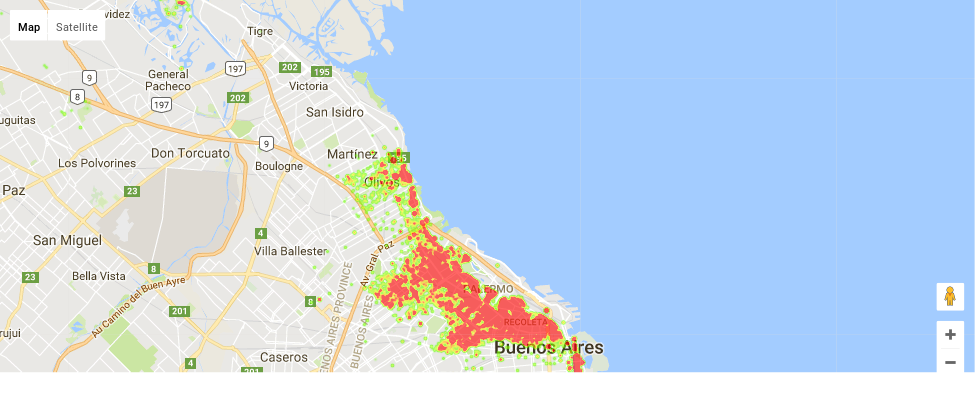
\includegraphics[width=\textwidth]{images/m2Group1HeatMap}
				  	\end{center}
				  	\tab En el gráfico se observa, más específicamente, que las propiedades con valores altos están ubicadas
				  	en el Este de la ciudad, esparciéndose desde el Microcentro hacia el Norte de CABA. Se puede ver, también,
				  	que las propiedades de la Provincia que se encuentran en este grupo son aquellas cercanas al río. Cabe destacar
				  	que Puerto Madero genera una 'discontinuidad' en el mapa, pues si se observa atentamente se ve que no está en
				  	una zona contigua al resto de los barrios. De todos modos, esto era de esperarse porque es un barrio construído
				  	específicamente como un 'lugar caro'. \\
				  	\tab Se debe mencionar, además, que el Barrio El Golf está ubicado en la localidad de Tigre y en este mapa no
				  	se lo puede ver. Se decidió dejarlo afuera para poder dar una mejor vista de la Capital Federal.
				\subsubsection{Grupo 2}
					Este segundo grupo se espera que esté compuesto por los barrios de capital y Zona Norte que no estaban presentes
					en el grupo previo. Esto es, San Isidro, Caballito, Saavedra, etc.
					\begin{center}
						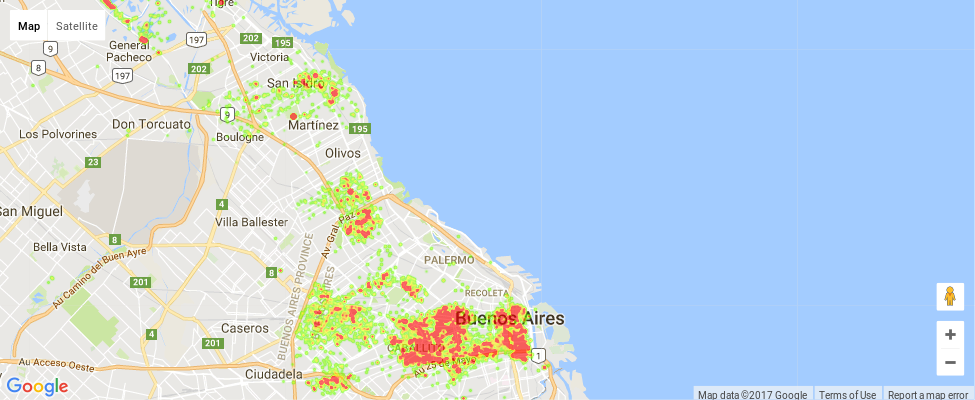
\includegraphics[width=\textwidth]{images/m2Group2HeatMap}
				  	\end{center}
				  	\tab El gráfico nos muestra que este segundo grupo contiene a los barrios del Sur Este de la Capital Federal
				  	('del centro para abajo', al revés que el grupo 1) y aquellos barrios que 'completan' la Zona Norte. Además, se
				  	encuentran algunos otros barrios dispersos, como por ejemplo Boedo. \\
				  	\tab Cabe destacar aquí también que en este segundo grupo se encuentran más barrios cerrados de la localidad de
				  	Tigre, como el Barrio Santa Bárbara y el Barrio Los Alisos, que nuevamente no se incluyeron en el mapa para
				  	poder dar más detalle a CABA.
				\subsubsection{Grupo 3}
					En este tercer grupo se espera que, además de que se cubra la mayor cantidad de superficie, se 'complete' la
					capital y comiencen a aparecer los barrios del llamado primer cordón del conurbano.
					\begin{center}
						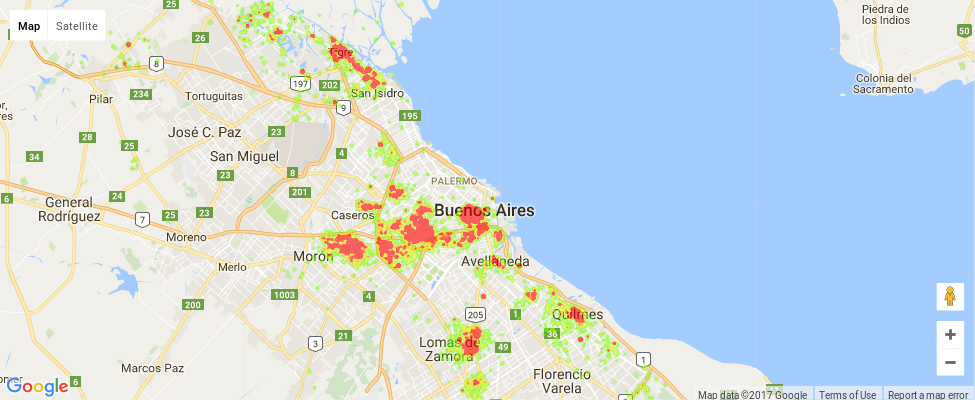
\includegraphics[width=\textwidth]{images/m2Group3HeatMap}
				  	\end{center}
				  	\tab El mapa presentado nos muestra, efectivamente, que está compuesto de los barrios restantes de la Capital
				  	Federal, algunos barrios del primer cordón, como Villa Martelli, Munro, Morón y otros más lejanos como Quilmes y
				  	Lomas de Zamora. Además, como se puede observar al Norte, se sigue completando la zona de barrios cerrados de la
				  	localidad de Tigre y sus alrededores. \\
				  	\tab También forma parte de este grupo la ciudad de La Plata pero se decidió dejarlo afuera de la visualización
				  	para poder enfocarnos más en CABA y GBA.
				\subsubsection{Grupo 4}
					Para este cuarto grupo, el segundo grupo principal como fue llamado previamente, se espera que se 'complete' el
					primer cordón del conurbano y comiencen a aparecer barrios del segundo y tercer cordón. También se espera que ya
					no aparezcan barrios de CABA.
					\begin{center}
						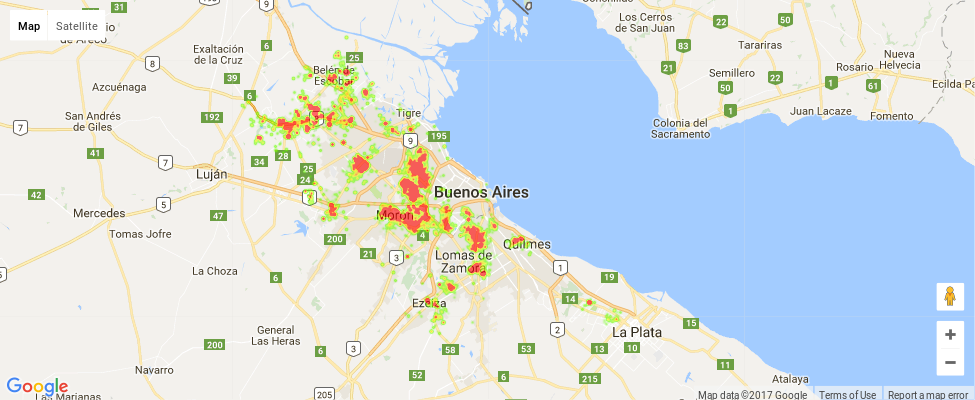
\includegraphics[width=\textwidth]{images/m2Group4HeatMap}
				  	\end{center}
				  	\tab En este caso se debió utilizar un nivel de zoom menor por la distancia entre los barrios del grupo. De todas
				  	maneras, se puede apreciar la aparición de más barrios del primer cordón del conurbano y de Pilar y Escobar, que
				  	son, al igual que Tigre, dos centros importantes de barrios cerrados y country clubs.
				\subsubsection{Grupo 5}
					Ya acercándonos a los barrios más baratos esperamos, tanto en este grupo como en el siguiente, encontrar
					barrios alejados de la Capital Federal pertenecientes al segundo y tercer cordón del conurbano.
					\begin{center}
						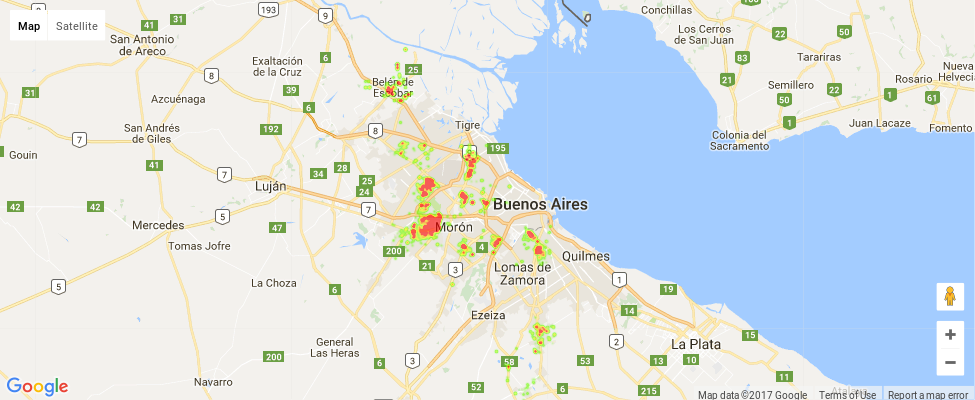
\includegraphics[width=\textwidth]{images/m2Group5HeatMap}
				  	\end{center}
				  	\tab Se puede observar que se completan algunas zonas faltantes del primer cordón del conurbano y aparecen zonas
				  	densas del segundo y tercer cordón, como se esperaba. De todas formas, al poseer cada vez menor cantidad de
				  	barrios, es más dificil hacer un mapa claro.
				\subsubsection{Grupo 6}
					Finalmente, en este sexto grupo esperamos encontrar barrios dispersos y alejados de la Capital Federal, con poca
					cantidad de propiedades.
					\begin{center}
						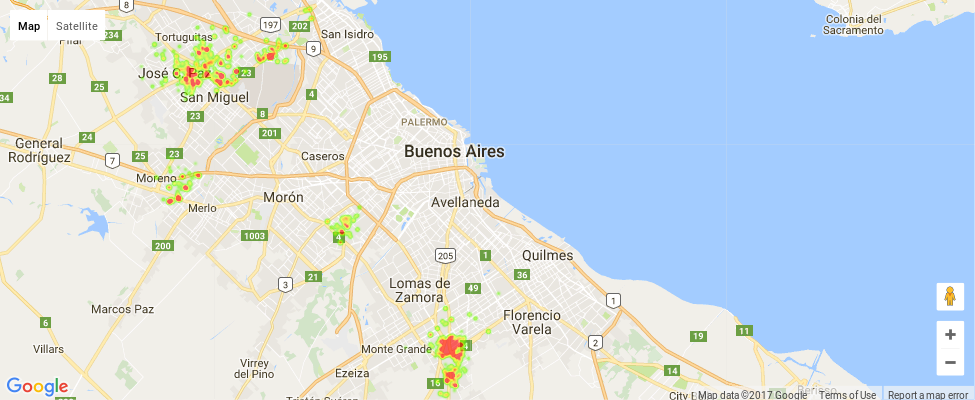
\includegraphics[width=\textwidth]{images/m2Group6HeatMap}
				  	\end{center}
				  	\tab Se verifica con este gráfico, entonces, que los integrantes de este último grupo pertencen al tercer,
				  	y más alejado, cordón del conurbano bonaerense.
				\subsubsection{Comparación de grupos}
					En este último gráfico mostraremos cómo se distribuyen los grupos en CABA y GBA, unificando todos los gráficos
					previos para un mejor entendimiento. Se utilizaron diferentes colores para diferenciar los grupos y dichos
					colores están indicados en la leyenda del gráfico.
					\begin{center}
						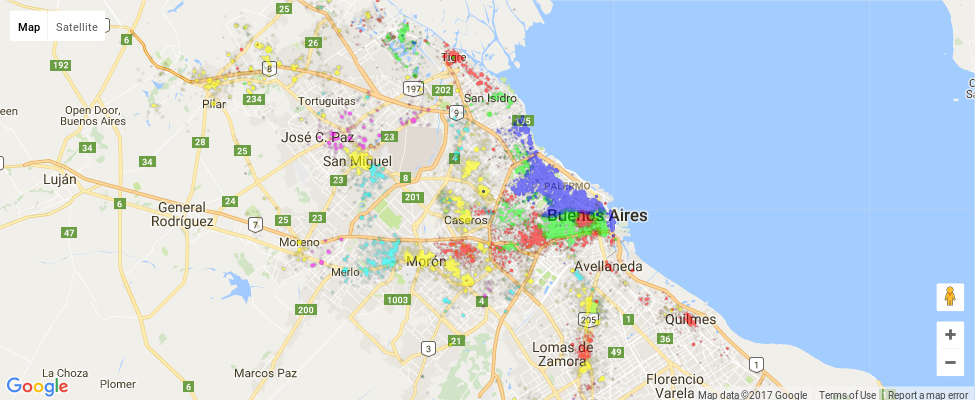
\includegraphics[width=\textwidth]{images/m2GroupComparison}
				  	\end{center}
				  	\tab NOTA: Grupo 1 AZUL, Grupo 2 VERDE, Grupo 3 ROJO, Grupo 4 AMARILLO, Grupo 5 CYAN, Grupo 6 MAGENTA.
				  	\emph{AGREGARLE LA LEYENDA A LA IMAGEN}
		\section{Progresión del precio por $m^2$ a través de los años}
			En esta sección se analizará como fue progresando el valor del $m^2$ entre los años 2013 y 2017. Para esto,
			se realizaron gráficos particulares para cada año como así también dos gráficos que comparan a todos los años entre sí.
			\subsection{Fluctuación del precio del $m2$ a través de los años}
				Para comenzar, se mostrará un gráfico en el que se muestra la variación del precio del $m^2$ entre el año 2013 y el 
				año 2017.
				\begin{center}
					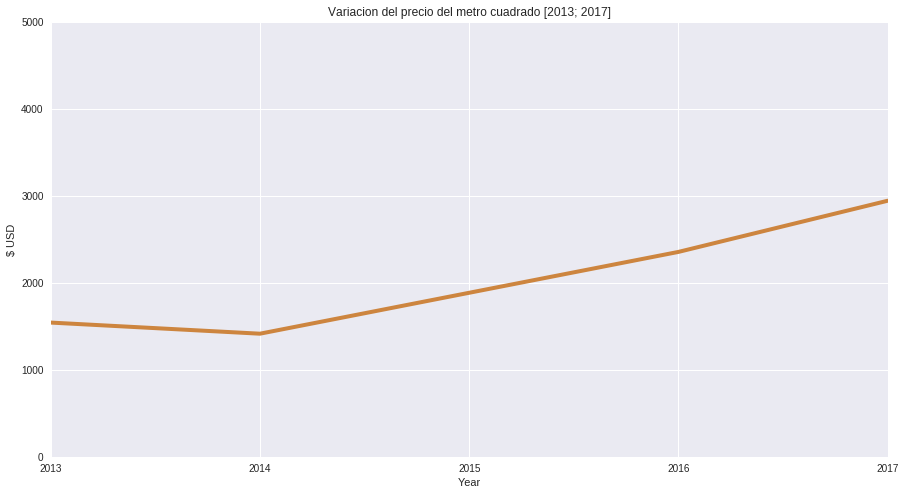
\includegraphics[width=\textwidth]{images/m2ProgressionGeneral}
				\end{center}
				\tab Se observa que entre 2013 y 2014 hubo un descenso del precio promedio pero que a partir de dicho año, el precio
				de las propiedades estuvo en aumento constante.
			\subsection{Año 2013}
				En este caso, se debe tener en cuenta que la cantidad de propiedad es la menor de todas y por lo tanto es posible
				que los precios disponibles no sean lo suficientemente representativos. De todas maneras, consideramos que es útil
				para un análisis comparativo con los años más recientes.
				\begin{center}
					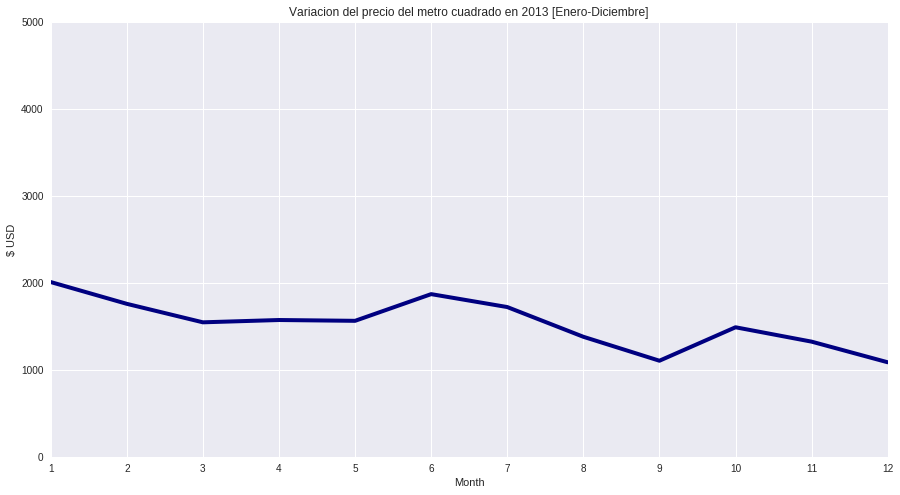
\includegraphics[width=\textwidth]{images/m2Progression2013}
				\end{center}
				\tab Se puede observar que el año 2013 tuvo una tendencia decreciente con aumentos sólo en los meses de Mayo
				y Septiembre.
			\subsection{Año 2014}
				Aquí la cantidad de propiedades ya es mayor, aunque muy menor a la de los años 2016 y 2017, de todas maneras, al
				igual que en el año anterior, es lo suficientemente descriptiva como para realizar una comparación más adelante.
				\begin{center}
					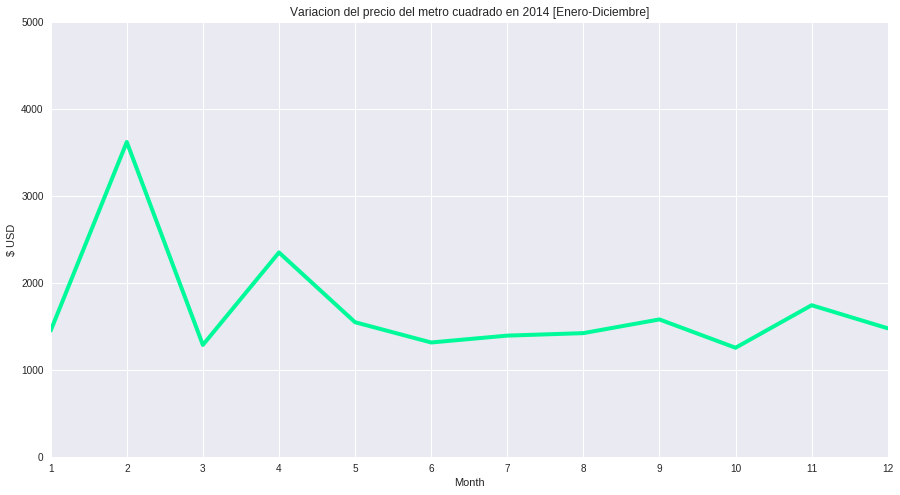
\includegraphics[width=\textwidth]{images/m2Progression2014}
				\end{center}
				\tab En este caso, vemos que hay una gran fluctuación de precios en los meses iniciales y finales pero se
				encuentra una región casi constante en los meses entre Mayo y Septiembre.  Podemos ver que, al igual que en 2013,
				el año termina con una baja del valor de $m^2$.
			\subsection{Año 2015}
				\begin{center}
					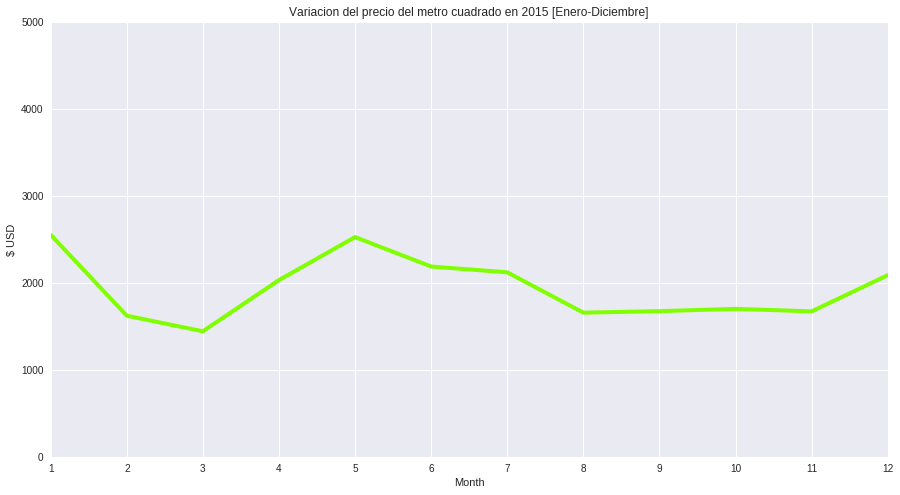
\includegraphics[width=\textwidth]{images/m2Progression2015}
				\end{center}
				\tab Podemos ver que este año comenzó con un decrecimiento del precio, luego volvió al precio de Enero y, luego de
				tres meses de precio constante, finalizó creciendo en Diciembre. Cabe destacar que el valor es bastante uniforme para
				los tres años hasta aquí analizados, aunque con un leve aumento.
			\subsection{Año 2016}
				\begin{center}
					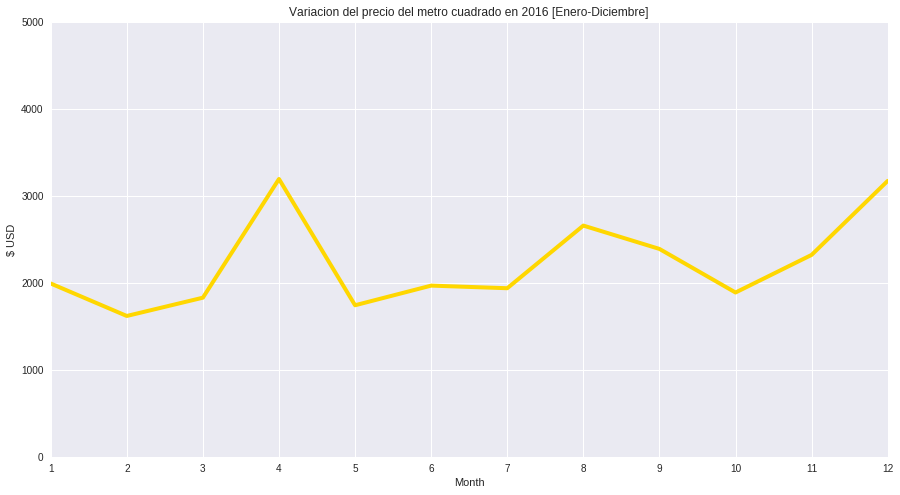
\includegraphics[width=\textwidth]{images/m2Progression2016}
				\end{center}
				\tab Este es, hasta aquí, el año con mayor fluctuación de precios. Con los decensos y ascensos más abruptos y con
				los valores más elevados. Se puede observar que el año finaliza con un aumento de precios muy importante, alcanzando
				el valor más alto hasta el momento.
			\subsection{Año 2017}
				Este es el año del que más información se posee, pues la información disponible es sobre publicaciones activas en
				la página oficial de \emph{Properati}. Obviamente, la información sólo llega hasta el mes de Agosto.
				\begin{center}
					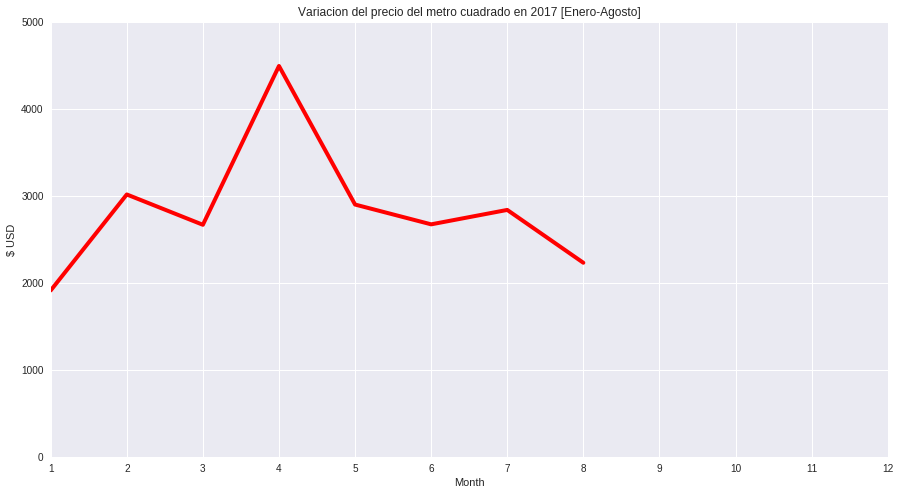
\includegraphics[width=\textwidth]{images/m2Progression2017}
				\end{center}
				\tab Aquí podemos ver que el año comenzó con un gran aumento, llegando a un pico de precios de los últimos cuatro
				años pero que, a partir del mes de Abril, comenzó el descenso y, para el mes de Agosto, ya casi se volvió a los
				valores de Enero.
			\subsection{Comparación de la progresión mensual en cada año}
				Ahora veremos dos gráficos en los que se unifica todo lo mostrado previamente, el cual nos permite comparar, año a
				año, cómo fue la variación de los precios. El primero es exactamente la superposición de los cuatro gráficos
				previos, mientras que el segundo (de barras) se utilizó para analizar mejor, mes por mes, en que año fue mayor
				el valor del $m^2$.
				\tab Comenzaremos analizando el mencionado gráfico de lineas:
				\begin{center}
					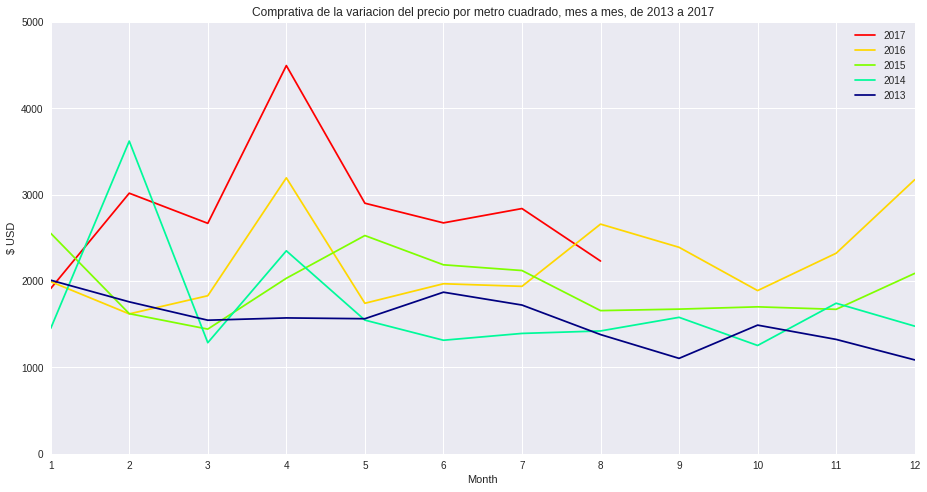
\includegraphics[width=\textwidth]{images/m2ProgressionLineComparison}
				\end{center}
				\tab Aquí podemos ver que el año 2017 (o al menos en lo que va del año) es el que mayores precios tiene en cinco de 
				los ocho meses en los que se posee información. Por otro lado, podemos ver que 2015 y 2016 terminan en suba mientras
				que 2013 y 2014 terminan en baja. También se puede ver que en los meses de Abril, Mayo y Junio hay una tendencia a
				suba de precios, mientras que no se encuentra una zona particular en la que haya tendencia a la baja de precios. \\
				\tab Ahora analizaremos el segundo gráfico, el de barras. El objetivo de este gráfico es, como se mencionó
				previamente, analizar, mes a mes, qué año tuvo los valores más altos.
				\begin{center}
					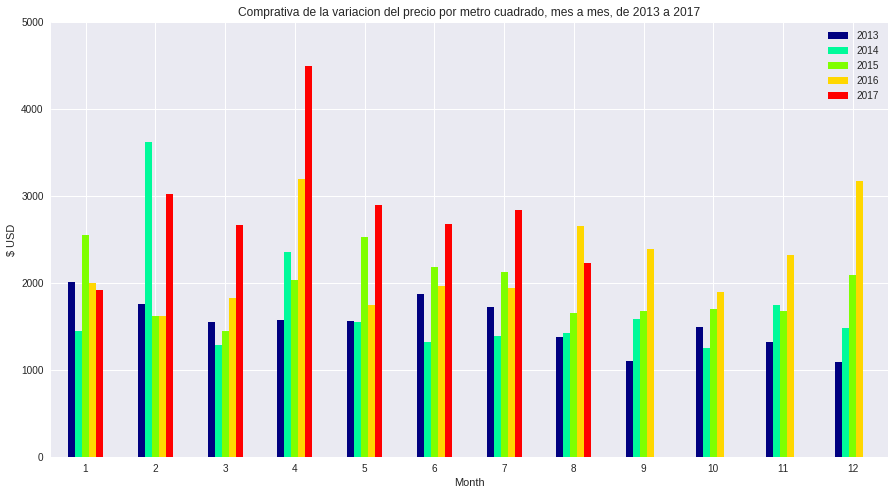
\includegraphics[width=\textwidth]{images/m2ProgressionBarComparison}
				\end{center}
				\tab Este gráfico permite ver que, si bien en 2017 se obtuvieron casi todos los valores récord en cada mes, mes a mes
				varía el orden de los años en cuanto a precio. Esto nos dice que los precios fluctuaron mucho en los últimos años
				aunque con una tendencia positiva (como ya vimos previamente), pues la mayoría de los máximos pertencen a años
				recientes.
		\section{Análisis de precio aproximado.}
	      	\subsection{Objetivo}
    				Esta sección tiene el objetivo de analizar como fueron variando los precios de las distintas propiedades en los
    				últimos 4 años. Con fin introductorio, se quiere brindar una mirada global acerca de la fluctuación de los precios
    				de todas las propiedades a lo largo de los últimos 4 años.
	      \subsection{Preparación y procesamiento de los datos}
			Para procesamiento de los datos, primero se separaron y agruparon los features por años. A continuación, para cada
			dataframe formado, es decir para las propiedades de un determinado año, lo que se hizo fue separarlas por meses. Entonces
			hasta el momento tenemos las propiedades separadas por años y por meses. Por último para cada año, se agruparon todas las
			propiedades de un mismo mes dejando como valor el precio en dolares promedio de las mismas. \\
       		\tab Por último, algo importante a tener en cuenta es que el set de datos esta referido a publicaciones y no a ventas de
       		propiedades en sí. Dichas publicaciones dejan de existir una vez que la propiedad fue vendida, por lo que los datos del
       		2013-2014 tal vez no sean lo suficientemente representativos por la cantidad de entradas que poseen, como si lo son los
       		datos del 2015 en adelante. De todas maneras, se usaron con fines representativos en el siguiente análisis. 

	      \subsection{Presentación de los gráficos de promedios}
	      	Aquí se muestran los gráficos que representan los promedios anteriormente mencionados para cada año. Vale aclarar que en
	      	los siguientes 5 gráficos el eje x representa los meses de cada año, y el eje y representa el precio de las propiedades
	      	en USD. Dicho precio varia entre 0$-$450000 $usd$, para obtener una mirada objetiva de los gráficos que serán presentados
	      	acontinuación.
			\begin{center}
       			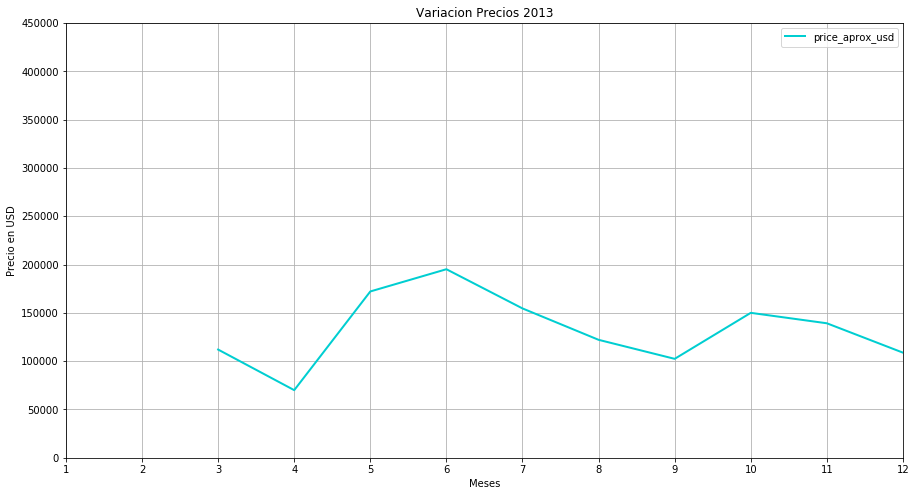
\includegraphics[width=6in, height=4.2in]{images/variacion2013}
		   	\end{center}
        		\begin{center}
       			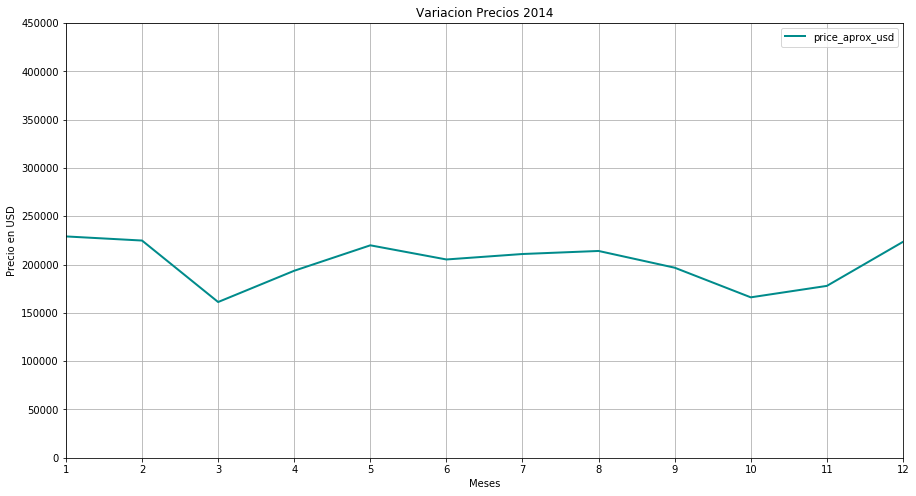
\includegraphics[width=6in, height=4.2in]{images/variacion2014}
		   	\end{center}
        		\begin{center}
       			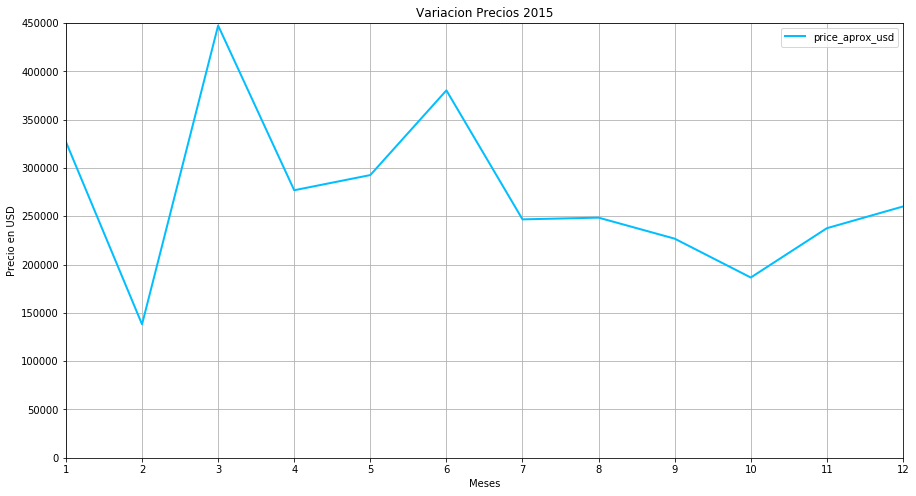
\includegraphics[width=6in, height=4.2in]{images/variacion2015}
		   	\end{center}
        		\begin{center}
       			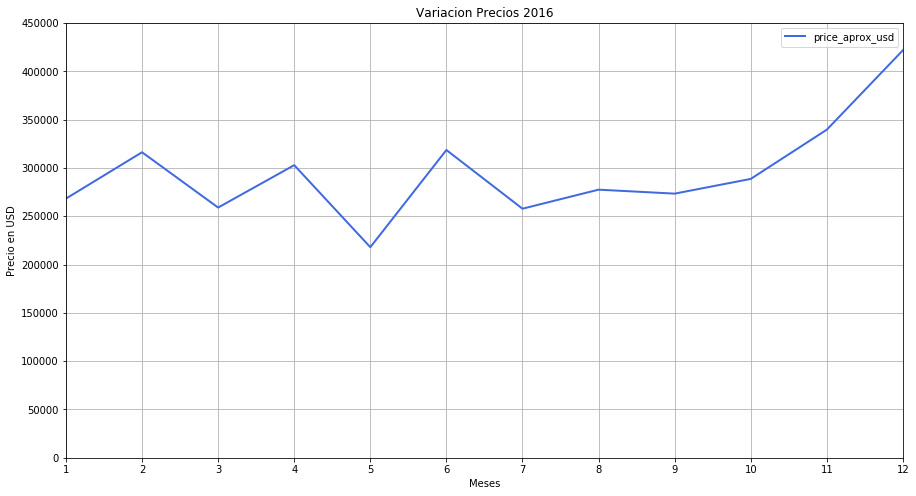
\includegraphics[width=6in, height=4.2in]{images/variacion2016}
		    \end{center}
        		\begin{center}
       			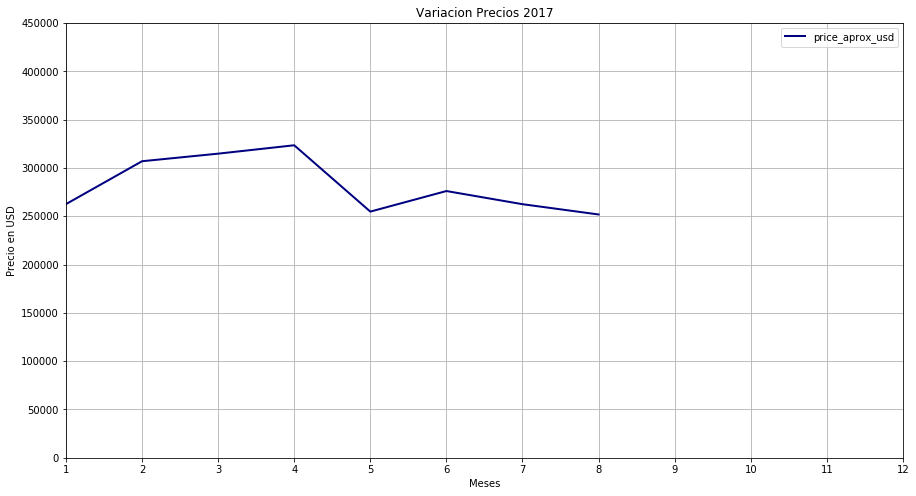
\includegraphics[width=6in, height=4.2in]{images/variacion2017}
		   	\end{center}

	      \subsection{Ubicación de las propiedades con mayor precio}
    			Luego de presentados los gráficos que representan la fluctuación del precio a través de los años, se procede a presentar
    			una serie de gráficos con el objetivo de analizar la ubicación de las propiedades con mayor precio. \\
 			\tab Para esto, se representa en distintos \code{Heats Map} la ubicación de las propiedades con mayor precio en cada año,
 			es decir que se filtro el mes que poseía un máximo en cada gráfico anterior y se representaron todas las propiedades que
 			estaban en dicho mes.
	        \begin{center}
    	         	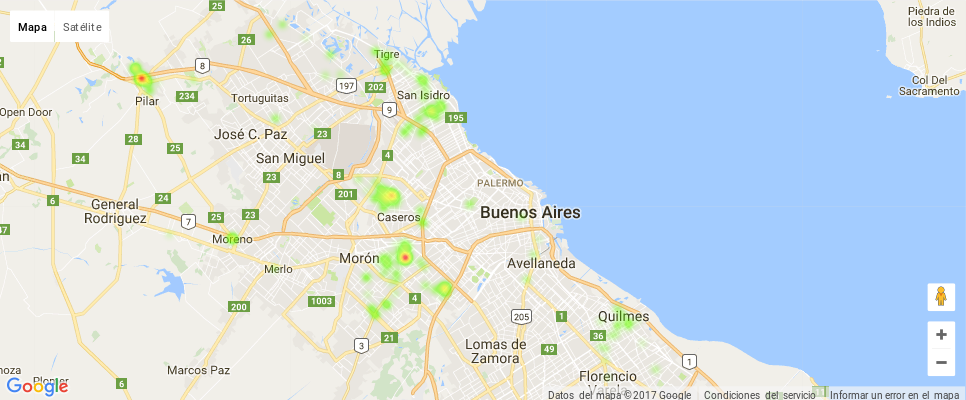
\includegraphics[width=7in, height=4in]{images/ubicP2013}
            		\textbf{Gráfico de las propiedades con mayor precio en el 2013.}
        		\end{center}
        		\begin{center}
              	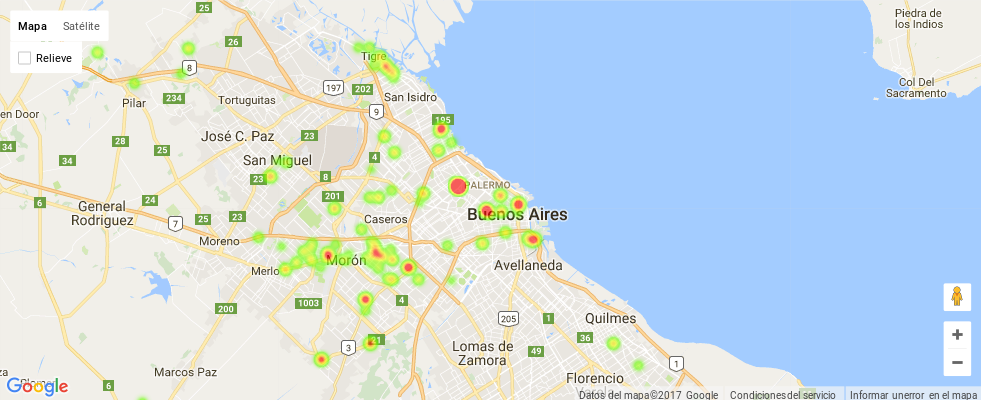
\includegraphics[width=7in, height=4in]{images/ubicP2014}
             	\textbf{Gráfico de las propiedades con mayor precio en el 2014.}
        		\end{center}
        		\begin{center}
             	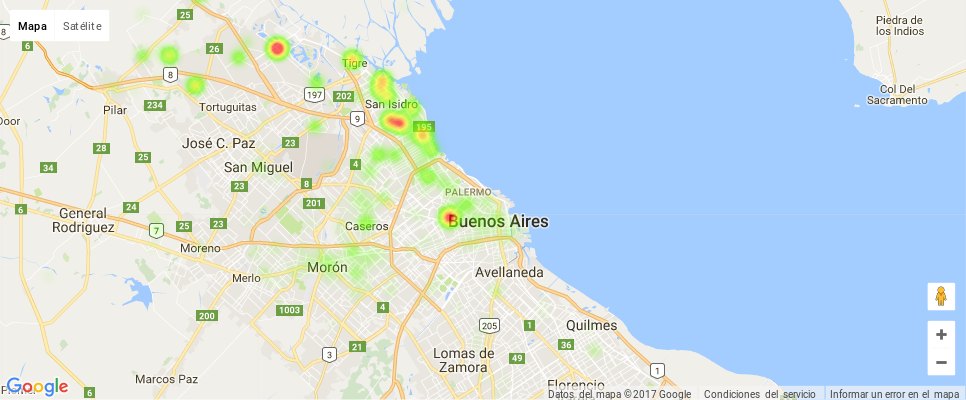
\includegraphics[width=7in, height=4in]{images/ubicP2015}
             	\textbf{Gráfico de las propiedades con mayor precio en el 2015.}
        		\end{center}
        		\begin{center}
              	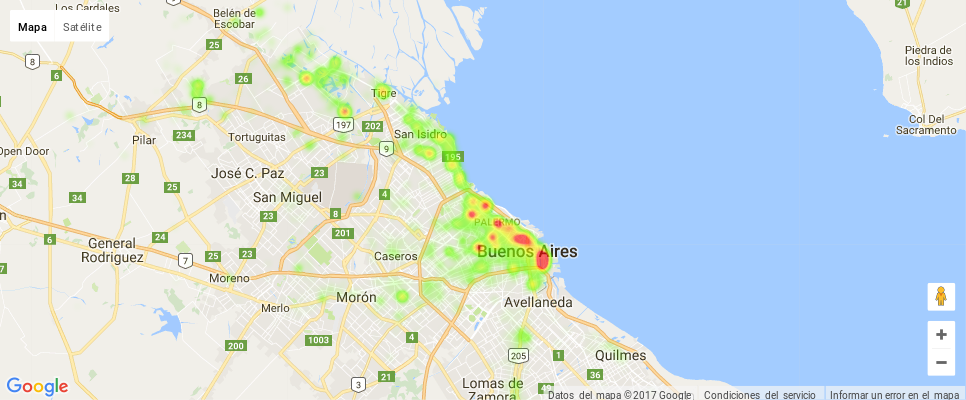
\includegraphics[width=7in, height=4in]{images/ubicP2016}
             	\textbf{Gráfico de las propiedades con mayor precio en el 2016.}
        		\end{center}
        		\begin{center}
              	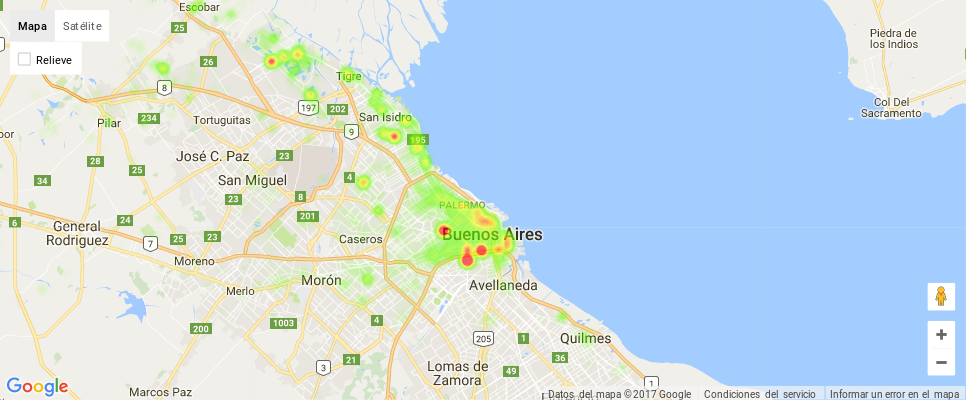
\includegraphics[width=7in, height=4in]{images/ubicP2017}
             	\textbf{Gráfico de las propiedades con mayor precio en el 2017.}
       		\end{center}
      	\subsection{Conclusiones de la Fluctuación del precio aproximado.}
			De los gráficos de promedios presentados anteriormente, se pueden visualizar rápidamente los meses con mayor y menor
			precio de propiedades en cada año. Se presenta una tabla con dichos datos:
        		\begin{center}
          		\begin{tabular}{ |c|c|c| }
            			\hline
		        		\multicolumn{3}{|c|}{Limites de precios por años.}\\
        		   		\hline
        		   		\hline
        		   		Año & Mes con Mayor Precio & Mes con menor Precio \\
        		   		\hline
        		   		2013 & Junio & Abril \\
        		   		2014 & Enero & Marzo \\
        		   		2015 & Marzo & Febrero \\
        		   		2016 & Diciembre & Mayo \\
        		   		2017 & Abril & Agosto \\
		            \hline
		        \end{tabular}
		    \end{center}
			\tab Cabe mencionar que estos son los datos que fueron filtrados para poder realizar los \code{Heats Map}. \\
	         \tab Por otra parte, se puede ver en la tabla presentada anteriormente que no se puede sugerir una tendencia de meses
	         con mayores-menores precios, ya que los resultados fueron muy variables. \\
	         \tab Con el objetivo de brindar otra mirada de la diferencia general entre los precios de distintos años, se construyó
	         otro gráfico que representa los mismo promedios anteriormente mencionados, pero organizados de distinta manera para
	         poder que puedan ser comparados entre distintos años. A continuación presentamos el gráfico:
			\begin{center}
              	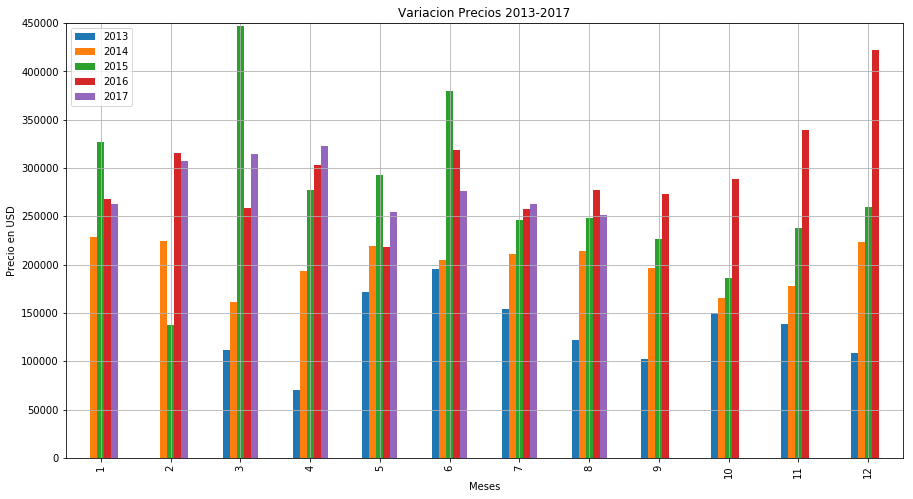
\includegraphics[width=6in, height=4.2in]{images/comparacionAnual}
        		\end{center}
        		\tab Como se menciono anteriormente, este gráfico tiene la finalidad de poder brindar una mirada global de los precios a
        		lo largo de los años. Como se puede ver, tenemos en el eje x los meses y para cada mes representamos los 5 años a
        		analizar. Observando detenidamente, se pueden extraer muchas conclusiones. \\
			\tab Lo primero y mas sencillo de ver son los meses con mayor y menor precio de los 5 años. Se puede observar que el 
			mes de Marzo del 2015 fue el que tuvo precios mas elevados de ventas, y por el contrario, el mes de Abril del 2013 
			fue el que tuvo los precios mas bajos en las mismas. Ademas se puede ver que 2013 tuvo menor precio que el resto de
			los años en todos los meses. Siguiendo la misma linea, es fácil observar que 2014 es el segundo año con menores precios,
			salvo en febrero que supero a 2015. De todas formas, se debe considerar que los años recientemente mencionados no son
			del todo representativos, ya que no se cuenta con la misma cantidad de datos que para los años posteriores.Por otro
			lado se puede visualizar que los primeros meses de 2015 fueron muy variantes, teniendo su mínimo en Febrero y máximo
			en Marzo, pero a partir de Junio-Julio se establece una media que supera a los 2 años anteriormente mencionados.
			Por último se puede ver que el año 2016 en la primera mitad posee precios que se sitúan entre los mas elevados, y
			en la segunda mitad establece una tendencia creciente la cual supera al resto de los años.
       		\tab A pesar de que los últimos años poseen un precio promedio mas elevado que los años previos, no se puede inferir
       		que haya aumentado el precio en el correr de los años, debido a la abrupta diferencia entre la cantidad de datos. De
       		todas formas, si solo es considerado el periodo 2015-2017, el cual posee la cantidad de entradas necesarias como para
       		ser representativo, obtenemos los siguientes resultados:
       		\begin{center}
       			\begin{tabular}{ |c|c| }
       			\hline
       			\multicolumn{2}{|c|}{Promedios Anuales de Precios.}\\
       			\hline
       			\hline
       			Año & Promedio(USD)\\
       			\hline
       			2015 & 292504 \\
       			2016 & 315746 \\
       			2017 & 275694 \\
       			\hline
	          	\end{tabular}
	      	\end{center}
     
			\tab De lo cual se puede ver rápidamente que el año 2016 fue el que tuvo precios mas elevados. De todas formas, hay
			que considerar que el año 2017 solo tiene entradas hasta agosto. \\
       		\tab Por otra parte, siguiendo el análisis recientemente hecho, se puede observar una cierta tendencia en los
       		\code{Heats Maps} presentados anteriormente. En dichos gráficos se puede notar que en los primeros años hay un
       		predominio de propiedades en \textit{Zona Norte} y \textit{Zona Oeste} del \textit{Gran Buenos Aires}. Esto puede
       		deberse, a la baja cantidad de entradas de dichos años, ya solo quedan las propiedades que no fueron vendidas.
       		Siguiendo con este análisis, se puede observar que los años posteriores poseen un mayor porcentaje de viviendas con
       		mayor precio en la zona de \textit{CABA}. Ademas, a esto le podemos sumar el análisis realizado en la sección 3.1,
       		sobre los barrios con mayor \code{Precio por m$^2$}. En ese análisis se obtuvo que los barrios con mayor valor de
       		metro cuadrado, están ubicados en \textit{CABA}, y mas precisamente, están ubicados en la zona que los últimos
       		2 \code{Heats Maps} nos indican mayor precio en las propiedades.
		\section{Conclusiones generales}
			Para finalizar esta parte, reflexionaremos sobre la información obtenida respecto del precio del $m^2$ en la Ciudad
			Autónoma de Buenos Aires y el Gran Buenos Aires. \\
			\tab Por empezar, es importante mencionar por qué esta es la parte uno; el precio del metro cuadrado será nuestra, por
			decir de alguna manera, \emph{unidad de medida} a lo largo de todo el trabajo. Por esta razón, parece correcto conocer
			cómo es que se distribuye en el espacio y cómo varió en los últimos años al inicio. \\
			\tab Conociendo la Ciudad de Buenos Aires y el momento actual del país, los resultados fueron los esperados. Es decir,
			la distribución espacial de los precios por $m^2$ es la esperada (disminuye a medida que nos alejamos de las conocidas
			'zonas caras' de la ciudad y describe a los llamados cordones del conurbano) y el precio en los últimos años tiene una
			tendencia creciente, tanto por $m^2$ como el precio total.
		\part{Análisis con Google Places}
		En este segmento se utilizo la API de Google Places 
		\footnote{https://developers.google.com/places/?hl=es-419} para obtener información adicional 
		sobre las propiedades provistas por Properati. Esta API permite entre otras cosas buscar 
		sitios (definidos en esta API como establecimientos, ubicaciones geográficas o puntos de 
		interés destacados) dentro de un área definida, como los límites de un mapa o alrededor de 
		un punto fijo. Para poder utilizarla sin embargo, se necesitan de coordenadas del tipo 
		latitud y longitud.\\ 
		El set de datos provistos contiene algunas ubicaciones en este formato pero no todas. 
		Por suerte dentro del set de datos está la información denominada como “geoname$\_$id”. 
		Este tipo de identificación pertenece a una base de datos geográfica con mas de 10 
		millones de entradas únicas. 
		Mediante la base de datos completa descargada de Kaggle
		\footnote{https://www.kaggle.com/geonames/geonames-database} se completaron las 
		latitudes y longitudes faltantes para así tener una muestra completa mayor.\\
		Para realizar pedidos a Google Places es necesario tener una API Key que esencialmente 
		controla el trafico diario de pedidos a la API. Esta limitación, utilizando una cuenta 
		prioritaria, es de 150000 pedidos por día. A la vez el tiempo entre que se realiza un 
		pedido y se obtiene su respuesta es muy alto. Es por esto que se limitaron las búsquedas 
		a las siguientes categorías(cantidades por propiedad en un radio de 400 metros):
		
		\begin{itemize}
		\item \emph{Locales de tipo gastronómico}
			\subitem Categorías de Google Places: \code{FOOD, BAKERY, BAR, MEAL$\_$TAKEAWAY, MEAL$\_$DELIVERY, RESTAURANT}
		\item \emph{Instituciones educativas}
			\subitem Categorías de Google Places: \code{SCHOOL, UNIVERSITY}
		\item \emph{Puntos de interés cultural} 
			\subitem Categorías de Google Places: \code{ART$\_$GALLERY, MUSEUM, PLACE$\_$OF$\_$WORSHIP}
		\item \emph{Espacios verdes} 
			\subitem Categorías de Google Places: \code{PARK, NATURAL$\_$FEATURE}
		\item \emph{Estaciones/Paradas de transporte publico}
			\subitem Categorías de Google Places: \code{BUS$\_$STATION, SUBWAY$\_$STATION}			
		\end{itemize}
		
		\section{Análisis Instituciones Educativas}
			\emph{A continuación se encuentra el análisis de las instituciones educativas para un set 
			de datos completo de 72474 entradas.}
			\subsection{Análisis del Precio por Metro Cuadrado}
				Para los siguientes gráficos se agruparon las propiedades por cantidad de instituciones 
				cercanas y sacando el promedio del precio por metro cuadrado para ellas. 
				Para que los resultados sean significativos, 
				se filtro a todas los conjuntos de propiedades con menos de 300 entradas para las 
				cantidades de instituciones cercanas. Por ejemplo: Si solo hay 15 propiedades con 
				60 instituciones cercanas, estas no se tuvieron en cuenta para el análisis.
				\begin{figure}
    				\centering
    				\makebox[\textwidth]{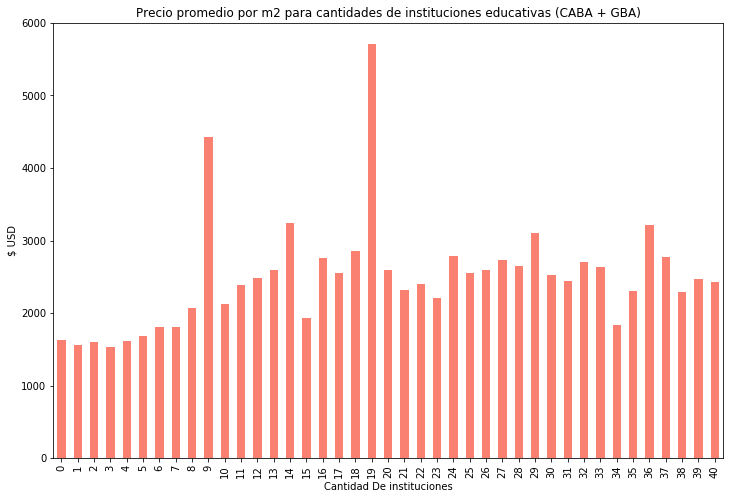
\includegraphics[width=\textwidth]{images/1}}
    				\caption{CABA + GBA}
				\end{figure}
				\begin{figure}
    				\centering
    				\makebox[\textwidth]{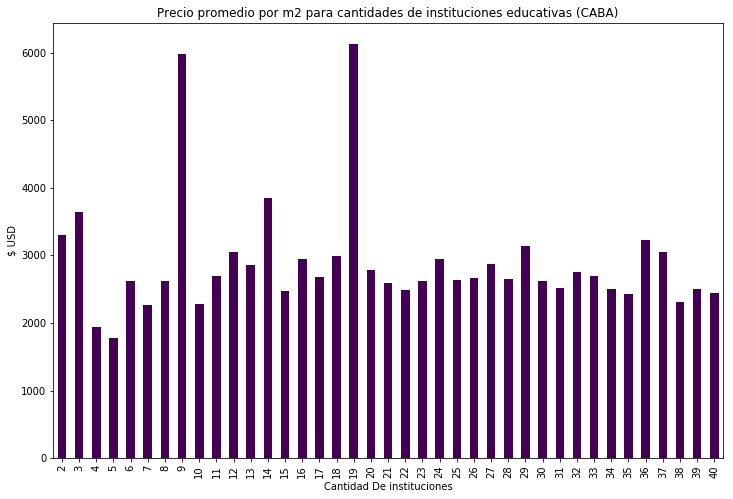
\includegraphics[width=\textwidth]{images/2}}
    				\caption{CABA}
				\end{figure}
				\begin{figure}
    				\centering
    				\makebox[\textwidth]{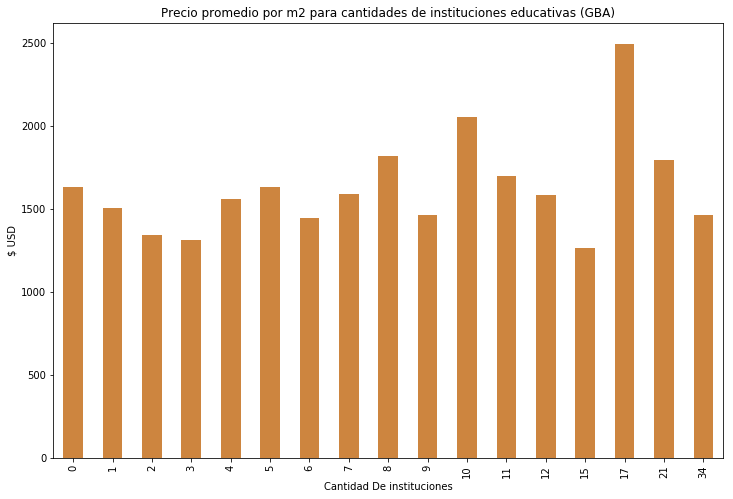
\includegraphics[width=\textwidth]{images/3}}
    				\caption{GBA}
				\end{figure}
				\FloatBarrier												
				
				Como se puede observar en los tres gráficos, hay una tendencia de un pico máximo 
				en todos para una cantidad de instituciones cercana a 20 instituciones. 
				Es importante notar sin embargo, que dichos máximos son muy distintos siendo el 
				de CABA casi el triple que el de GBA (6000 contra 2400 respectivamente).\\
				Se procede a aislarlas y observar en que zonas se concentran.\\
				
				\begin{figure}
    				\centering
    				\textbf{HEATMAP por ubicaciones}\par\medskip
    				\makebox[\textwidth]{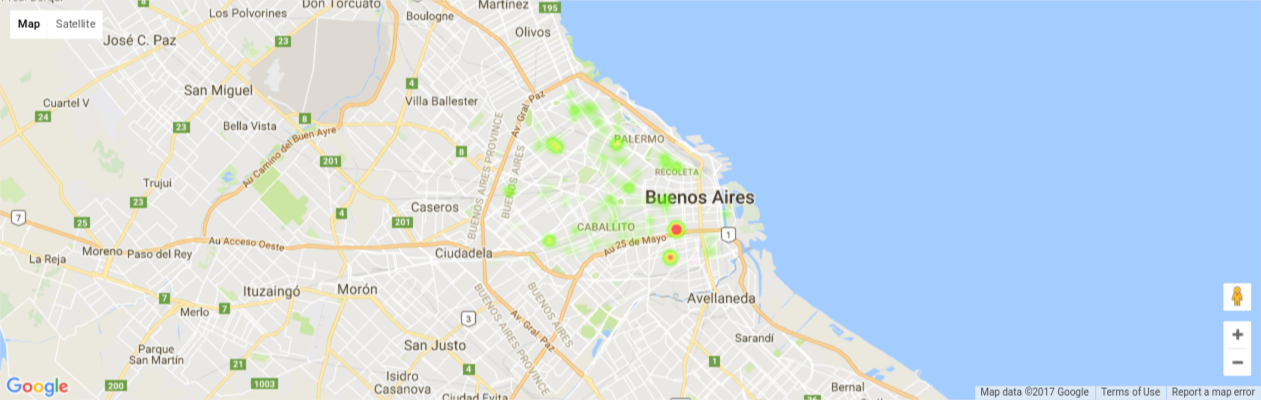
\includegraphics[width=\textwidth]{images/4}}
    				\caption{CABA con 19 instituciones}
				\end{figure}				
				\begin{figure}
    				\centering
    				\textbf{HEATMAP por precio del metro cuadrado}\par\medskip
    				\makebox[\textwidth]{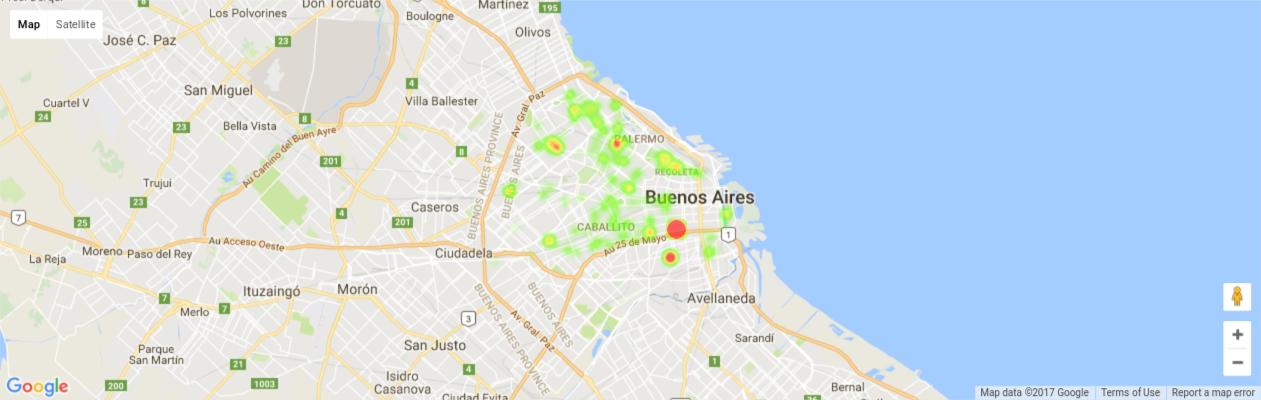
\includegraphics[width=\textwidth]{images/5}}
    				\caption{CABA con 19 instituciones}
				\end{figure}				
				\begin{figure}
    				\centering
    				\textbf{HEATMAP por ubicaciones}\par\medskip
    				\makebox[\textwidth]{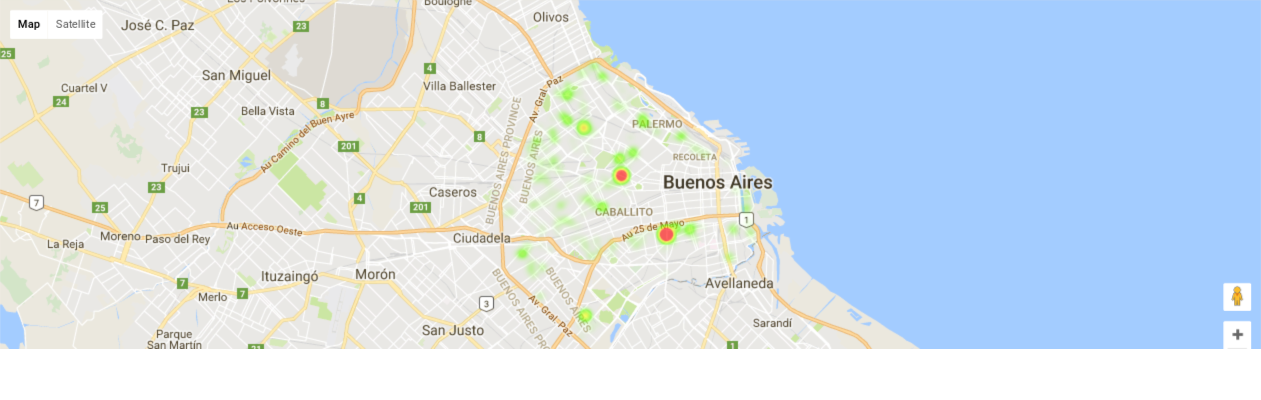
\includegraphics[width=\textwidth]{images/6}}
    				\caption{CABA con 9 instituciones}
				\end{figure}				
				\begin{figure}
    				\centering
    				\textbf{HEATMAP por precio del metro cuadrado}\par\medskip
    				\makebox[\textwidth]{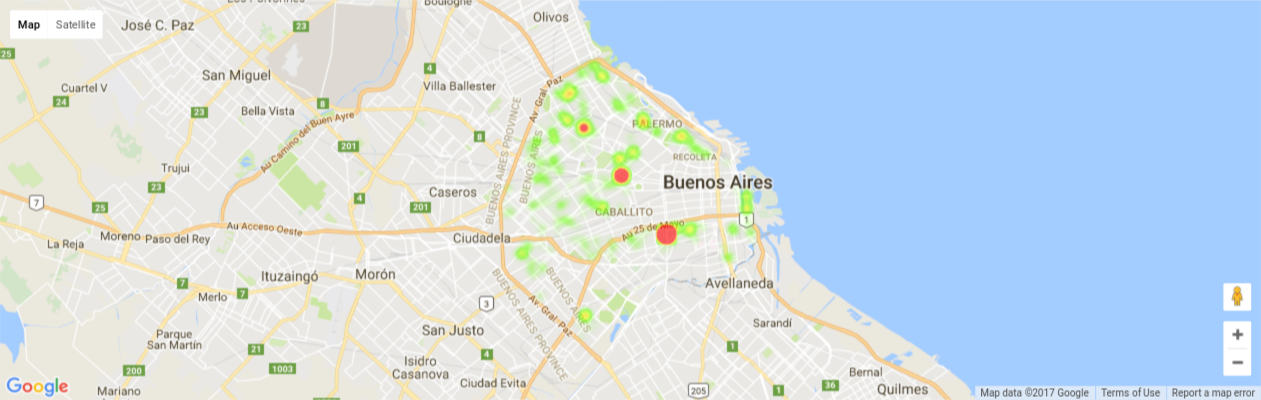
\includegraphics[width=\textwidth]{images/7}}
    				\caption{CABA con 9 instituciones}
				\end{figure}				
				\begin{figure}
    				\centering
    				\textbf{HEATMAP por ubicaciones}\par\medskip
    				\makebox[\textwidth]{\includegraphics[width=\textwidth]{images/8}}
    				\caption{GBA con 17 instituciones}
				\end{figure}
				\begin{figure}
    				\centering
    				\textbf{HEATMAP por precio del metro cuadrado}\par\medskip
    				\makebox[\textwidth]{\includegraphics[width=\textwidth]{images/9}}
    				\caption{GBA con 17 instituciones}
				\end{figure}
				\FloatBarrier

				\textbf{¿Que conclusiones se obtienen de estos heatmaps?}\\	
					\tab Se pueden ubicar polos en donde hay una cantidad importante de instituciones educativas 
					(entre 17 y 20 en un rango de 400 metros de radio) y a la vez los precios por metro 
					cuadrado son altos en comparación a la totalidad de las propiedades. En ellos se 
					genera una tendencia que podría marcar una relación directa entre estos dos factores.\\ 
					Estos lugares son:
					\begin{itemize}
					\item Olivos
					\item San Cristóbal
					\item Villa Urquiza/General Urquiza
					\item Parque Patricios
					\item Colegiales
					\end{itemize}						

					A menor escala, zonas céntricas de los siguientes barrios:
					\begin{itemize}
					\item Merlo
					\item San Miguel
					\item Quilmes
					\item Recoleta
					\item Belgrano
					\item Puerto Madero
					\item Almagro
					\end{itemize}


					Resulta interesante notar una situación particular que ocurre en lugares como Villa Crespo 
					y Boedo en donde el promedio de instituciones cercanas es 9 pero sin embargo hay precios 
					muy altos en las propiedades. Esto genera una problemática en cuanto a la validez del 
					análisis por instituciones educativas y sugiere quizás realizar un filtro mas estricto 
					en los datos para futuros análisis. Sin embargo 10 instituciones educativas en un 
					rango de 400 metros sigue siendo un numero importante.\\
					
				\textbf{¿Cuales son las instituciones educativas en estos polos?}\\
					\tab A continuación se muestran los nombres de dichas instituciones por barrio
					(Solo de los 3 barrios mas significativos) para tenerlas en cuenta en 
					futuros análisis cuando se busque predecir precios por propiedades. 
					Cabe aclarar que son mas de 20 ya que se toman el conjunto de todas 
					las instituciones del barrio y no solo las de una ubicación en particular.\\
					
					\emph{\textbf{Olivos:}}
					\begin{itemize}
					\item Northlands
\item Colegio San Andrés secondary
\item Centro Cultural Italiano - Colegio Alessandro Manzoni
\item St. Andrew's Scots School
\item Instituto Jesús en el Huerto de los Olivos
\item Escuela Montessori Olivos SRL
\item Colegio San Ignacio
\item Colegio Nuestra Señora de la Paz
\item St. Luke's College
\item Action Integral Institute of Performing Arts
\item Escuela Municipal Paula Albarracín de Sarmiento
\item San Andres Secundario Olivos
\item St. Nicholas College
\item Instituto Superior De Musica Jose Hernandez
\item Escuela EPB Nº 2 “Benemérito Teniente Gral. Bartolomé Mitre”
\item UCES OLIVOS
\item Colegio Tarbut
\item Estudio Cambrée Tatiana Flaker
\item UCES UNIVERSITY OF BUSINESS AND SOCIAL SCIENCES
\item Fundacion Universidad de San Isidro
\item Colegio San Nicolas Primario
\item COLEGIO SAN NICOLAS JARDIN
\item Escuela Superior De Informatica De La Prefectura Naval Argentina
\item CENTRO PAMPA / escuela de diseño
\item Colegio Santa Magdalena
\item Colegio Eidep
\item De Los O Colegio Jesus En El Huerto
\item Jardin San Ignacio
\item E.M.P.A.S
\item Ganesha YOGA
\item Colegio Feli
\item Escuela Hija St Andrews
\item Auditorio niño Jesus De Praga
\item Escuela Municipal De Musica
\item Niño Jesús Del Praga
\item Jardín Maternal Niño Jesús de Praga
\item Auditorio Northlands School Olivos
\item Escuela De Tomas, Francisco Borges Y Rosales
\item Jardin Jho
\item Jardin de infantes CCI - Centro Cultural Italiano -
\item Jardin centro cultural italiano
\item Colegio Centro Cultural Italiano
\item SCUOLE CCI
\item Jardin Jesus en el Huerto de los Olivos
\item Jardin Dante
\item ArtBA
\item ITBA
\item Jardin Maternal Osecac
\item Instituto San Migue
\item St. Nicholas College
\item English Boutique
\item Scout Huerto De Los Olivos
\item Grupo Capoeira Brasil Buenos Aires GCB - La Lucila
\item CID vicente lopez
\item Colegio Nuestra Sra De La Paz
\item Toefl
\item Centro Cultural y Político Micaela García
\item Centro de Instrucción Aeronáutica C.I.A.
\item Escuela N 16 Marcelino Ugarte
\item Escuela EST Nro 3
					\end{itemize}				
					\emph{\textbf{San Cristóbal:}}
					\begin{itemize}
					\item DE LAS VICTORIAS
\item La Aldea del Buen Ayre
\item Instit Salesiana - Colegio San Antonio
\item Escuela Generación del Futuro
\item Danza Árabe Escuela Aldana Arguello
\item Sol de America
\item Crema y Chocolate
\item Crema y Chocolate
\item Fundacion tomas eloy martinez
\item Curso de cerrajerìa presencial e intensivo
\item Cenedi
\item AUDITORIO NAMUNCURA
\item Colegio San José de Calasanz
\item Colegio Calasanz
\item San Antonio
\item ILEC - Instituto Laico de Estudios Contemporaneos
\item Special Education Institute OUR LADY OF LUJAN
\item Curso Sublimacion
\item Escuela Domiciliaria N 2
\item JIC N 4 DE 6 MARIANO BOEDO
\item Ciber Pibes
\item Escuela Infantil Cyberpibes
\item Instructorado De KIZOMBA
\item Esc de Com Nº 22 DE 6 "G. M. Zubiria "
\item Espacio De Creacion Yapeyu
\item ESCUELA N. 6 D.E. 8 SAN JOSÉ DE CALASANZ
\item Escuela N 25 Paula A De Sarmiento
\item Pasillo al fondo "Centro Cultural"
\item Instituto Calazans
\item Escuela Lucia
\item ESCUELA PAULA ALBARRACIN DE SARMIENTO
\item Escuela Infantil La Torrecita
\item "Puente Azul" Jardín de Infantes
\item Taller De Arte Hilodearbol
\item San Antonio Salesian house
\item Curso Calidad
\item SANTA MARIA INSTITUTE
\item Instituto San Antonio-A.226
\item Escuela De TANTRACLASICO
\item CFP No.30
\item Yoga
\item Escuela No9 D.E. 8 - Florentino Ameghino
\item Supervision D E 8 Primaria
					\end{itemize}
					\emph{\textbf{Villa Urquiza/General Urquiza:}}
					\begin{itemize}
					\item School No. 24 Francisco Morazan
\item San Patricio Secondary Institute
\item Nuevos Aires SRL
\item Sir Thomas Malory
\item Mad Escuela
\item Sir Thomas Malory School
\item Estudio Joya
\item Instituto Superior del Profesorado en Educación Especial
\item INA - Instituto Nuevos Aires
\item St. Patrick's School
\item Escuela Infantil Chiquilines
\item Instituto Junín
\item The Garden of the Fund
\item Special Education School 11
\item Burdel de maderas
\item Clases de Guitarra en Villa Urquiza - Música y creatividad
\item St. Patrick's School instituto San Patricio
\item Saint Patrick
\item Acha Club
\item Caebt 56 - Parroquia Jesús Misericordioso
\item St patrick's Kinder
\item Naranon grupo
\item Escuela Nro. 4 D.E. 15
\item Escuela Nro 24 D.E.15 - Escuela Nro 8
\item Ispee
\item Facu Aye
\item Facultad Moron
\item ESc Infantil N 8 DE 15
\item San Pablo
\item Island of My Dreams
\item escuela republica de costa rica
\item Escuela No 24 SIGLO XXI
\item Escuela n•15 acevedo
\item Universidad -ciclo basico
\item Drago Uba
\item CBC Drago
\item Colegio Franco
\item UBA - Drago
\item UBA Sede Drago
\item Cbc
\item CBC UBA - Sede Drago
\item Sede Drago
					\end{itemize}
					
					Es importante notar, como se puede ver en las ultimas instituciones de 
					Villa Urquiza, la sede Drago del CBC aparece subida repetidas veces 
					pero escrita de distinta manera. Esto muestra que mas allá del gran 
					poder que tiene Google Places, los datos pueden no ser del todo fehacientes.
					
		\subsection{Análisis de la Superficie Total de la Propiedad en Metros Cuadrados} 
			A partir de este análisis se busca encontrar alguna relación entre el tamaño de la propiedad 
		y la cantidad de instituciones en su cercanía. Previo a los resultados se supone que puede 
		llegar a haber una relación teniendo en cuenta que mientras mas grande sea, es mas probable 
		que mas personas vivan allí y por consiguiente necesiten de variadas instituciones educativas. 
		A la vez se podría dar también que pequeñas propiedades estén en zonas donde la demanda de 
		instituciones educativas se muy alta y por esta razón priorizar la cercanía a las instituciones 
		dejando de lado otras comodidades como puede ser un mayor espacio.			
		
				\begin{figure}
    				\centering
    				\makebox[\textwidth]{\includegraphics[width=\textwidth]{images/10}}
    				\caption{CABA + GBA}
				\end{figure}
				\begin{figure}
    				\centering
    				\makebox[\textwidth]{\includegraphics[width=\textwidth]{images/11}}
    				\caption{CABA}
				\end{figure}
				\begin{figure}
    				\centering
    				\makebox[\textwidth]{\includegraphics[width=\textwidth]{images/12}}
    				\caption{GBA}
				\end{figure}
				\FloatBarrier
				
				Al darle una vista rápida a los gráficos se  ven que los comportamientos de 
				CABA Y GBA son muy distintos. Pero en este caso los picos máximos tienen 
				valores similares rondando entre 500 y 600 metros cuadrados. 
				Se procede a analizar los datos por separado para obtener conclusiones mas precisas.\\
				
				\textbf{¿Que conclusiones se obtienen de GBA?}\\
				En GBA se ve una tendencia a la baja de tamaños, siendo que a mayor 
				cantidad de instituciones, las propiedades tienen un tamaño menor. 
				Una posible razón puede adjudicarse a que muchas de las propiedades 
				de GBA pertenecientes al Dataframe son de barrios cerrados en donde 
				los terrenos suelen ser particularmente grandes y a la vez las 
				distancias a, no solo instituciones educativas si no también a 
				locales o zonas con mayor población, son superiores.\\
				
				\textbf{Relación entre el tamaño total de la superficie y la cantidad de 
				instituciones educativas para CABA}\\
				Se distinguen dos claros picos máximos en 5 instituciones, y en 38. 
				Mas allá de esto no se ven otras relaciones que resulten de interés 
				para el análisis. Para ubicar las propiedades en cuestión se realiza 
				un heapmap con ellas.
					
				\begin{figure}
    				\centering
    				\textbf{HEATMAP por ubicaciones}\par\medskip
    				\makebox[\textwidth]{\includegraphics[width=\textwidth]{images/13}}
    				\caption{CABA con 5 instituciones}
				\end{figure}				
				\begin{figure}
    				\centering
    				\textbf{HEATMAP por tamaño de superficie}\par\medskip
    				\makebox[\textwidth]{\includegraphics[width=\textwidth]{images/14}}
    				\caption{CABA con 5 instituciones}
				\end{figure}				
				\begin{figure}
    				\centering
    				\textbf{HEATMAP por ubicaciones}\par\medskip
    				\makebox[\textwidth]{\includegraphics[width=\textwidth]{images/15}}
    				\caption{CABA con 38 instituciones}
				\end{figure}				
				\begin{figure}
    				\centering
    				\textbf{HEATMAP por tamaño de superficie}\par\medskip
    				\makebox[\textwidth]{\includegraphics[width=\textwidth]{images/16}}
    				\caption{CABA con 38 instituciones}
				\end{figure}				
				\FloatBarrier
				
				\textbf{¿Que conclusiones se obtienen de estos heatmaps?}\\
				En los heatmaps con 5 propiedades en CABA se marca la tendencia que ubicaba a 
				Villa Crespo como un polo. En donde hay una base solida pero no muy grande de 
				instituciones educativas y a la vez hay precios altos por metro cuadrado y 
				propiedades de tamaños importantes. A esto se agrega la zona de puerto madero 
				en donde se observan precios muy altos, grandes propiedades, y un buen numero 
				de instituciones educativas, particularmente universidades.\\
				Finalmente se ubican dos nuevos polos con propiedades muy grandes y realmente un numero 
				enorme de instituciones (38 instituciones) siendo estos Plaza Dorrego y en Flores cerca 
				de la Av. Rivadavia entre Av.Nazca y Av.Carabobo.
		\section{Análisis de Locales Gastronómicos}
			\emph{A continuación se encuentra el análisis de las instituciones de tipo gastronómicas para 
			un set de datos completo de 72474 entradas.}
			\subsection{Análisis del precio por metro cuadrado}
				Para los siguientes gráficos se agruparon las propiedades por cantidad de instituciones 
				cercanas y sacando el promedio del precio por metro cuadrado para ellas. 
				Para que los resultados sean significativos, se filtro a todas los conjuntos 
				de propiedades con un precio menor a \textdollar USD8000 teniendo en cuenta 
				el análisis inicial.
				
				\begin{figure}
    				\centering
    				\makebox[\textwidth]{\includegraphics[width=\textwidth]{images/17}}
    				\caption{CABA + GBA}
				\end{figure}
				\begin{figure}
    				\centering
    				\makebox[\textwidth]{\includegraphics[width=\textwidth]{images/18}}
    				\caption{CABA}
				\end{figure}
				\begin{figure}
    				\centering
    				\makebox[\textwidth]{\includegraphics[width=\textwidth]{images/19}}
    				\caption{GBA}
				\end{figure}
				\FloatBarrier
				
				A simple vista los gráficos no dicen mucho. Es observable una leve tendencia de 
				crecimiento en cuanto a mayor cantidad de locales el precio de las propiedades 
				seria mayor y lo mismo para menor cantidad de locales. Dicha tendencia se puede 
				apreciar mejor en el gráfico de GBA + CABA. En los otros gráficos, la tendencia 
				de punta a punta (mas allá de abruptas variaciones) se asemeja a constante.  
				Se procede a ubicar donde están los lugares con menores locales y donde están 
				los que mas tienen, es decir, los extremos.
				
				\begin{figure}
    				\centering
    				\textbf{Heatmap con el peso en el precio por metro cuadrado de locales gastronómicos}\par\medskip
    				\makebox[\textwidth]{\includegraphics[width=\textwidth]{images/20}}
    				\caption{CABA + GBA de 0 a 20 locales}
				\end{figure}				
				\begin{figure}
    				\centering
    				\textbf{Mismo Heatmap que la figura anterior pero con ZOOM}\par\medskip
    				\makebox[\textwidth]{\includegraphics[width=\textwidth]{images/21}}
    				\caption{CABA + GBA de 0 a 20 locales}
				\end{figure}
				\FloatBarrier				
				
				De estos últimos heatmaps se puede extraer la interesante conclusión de que 
				las propiedades con pocos locales gastronómicos a su alrededor pertenecen a 
				GBA y prácticamente excluyen a CABA.				
								
				\begin{figure}
    				\centering
    				\textbf{Heatmap con el peso en el precio por metro cuadrado de locales gastronómicos}\par\medskip
    				\makebox[\textwidth]{\includegraphics[width=\textwidth]{images/22}}
    				\caption{CABA + GBA de 180 a 200 locales}
				\end{figure}								
				\FloatBarrier
				
				Continuando con el análisis previo, las propiedades con entre 180 y 200 
				locales gastronómicos en sus cercanías están en su totalidad ubicados en CABA, 
				mas particularmente su zona céntrica.\\
				
				\textbf{Principales polos gastronómicos}\\
				Analizando mas detalladamente las posiciones de las propiedades 
				en el mapa se encuentran los siguientes sectores como principales polos gastronómicos:
\begin{itemize}
	\item Plaza Serrano
	\item Recoleta
	\item Plaza Dorrego
	\item Belgrano
\end{itemize}


				Cabe aclara que en GBA las mayores concentraciones están ubicadas en la 
				cercanía de centros comerciales (shopping centers).
	
		\section{Análisis de Puntos de Interés Cultural}
			\emph{A continuación se encuentra el análisis de los puntos de interés cultural 
			para un set de datos completo de 72474 entradas.}
			
			\subsection{Análisis del precio por metro cuadrado}
				Primero se comienza sin agregar ningún recorte extra al set de datos y se 
				analiza una descripción del set de datos. Utilizando la función describe, 
				es posible notar que menos del \%50 de los datos tienen una cantidad de 
				entradas menor a 60. Esto quiero decir que puede haber por ejemplo solo 
				una propiedad con un numero muy alto de entradas que distorsiones a todo 
				el resto. Como lo que se esta tratando de buscar son tendencias. 
				Se procede a cortar la cantidad de instituciones por el porcentual del \%99 
				para achicar posibles disrupciones. 
				Finalmente recortando por cantidad de puntos culturales menores a 65 y 
				que estos tengan por lo menos 10 repeticiones se obtienen los siguientes gráficos:

				\begin{figure}
    				\centering
    				\makebox[\textwidth]{\includegraphics[width=\textwidth]{images/23}}
    				\caption{CABA + GBA}
				\end{figure}
				\begin{figure}
    				\centering
    				\makebox[\textwidth]{\includegraphics[width=\textwidth]{images/24}}
    				\caption{CABA}
				\end{figure}
				\begin{figure}
    				\centering
    				\makebox[\textwidth]{\includegraphics[width=\textwidth]{images/25}}
    				\caption{GBA}
				\end{figure}
				\FloatBarrier
				
				Instantáneamente se percibe lo que conociendo el territorio seria sospechable. 
				Esto es en primer medida que la cantidad de puntos de interés cultural en 
				CABA contra los de GBA es considerablemente mayor siendo 49 contra 14 las 
				respectivas cantidades máximas. A la vez es notable resaltar que en gráfico 
				de CABA + GBA hay una clara disminución en el precio de la propiedad para 
				lugares con 0 o 1 puntos cercanos. Mas allá de estos conceptos, los tendencias 
				sugieren ser a simple vista constantes.\\ 
				\tab Se trata de ubicar a las propiedades con pocos puntos cercanos en zonas particulares.						 					
				\begin{figure}
    				\centering
    				\textbf{Heatmap con el peso en las ubicaciones}\par\medskip
    				\makebox[\textwidth]{\includegraphics[width=\textwidth]{images/26}}
    				\caption{CABA + GBA con 0 o 1 puntos de interés cultural cerca}
				\end{figure}				
				\FloatBarrier
				
				Como los gráficos anticipaban, casi en su totalidad estas propiedades están ubicadas en GBA. 
				Sin embargo surge un punto interesante y es que se concentran mas que nada en la zona 
				norte de GBA. Esto podría adjudicarse a que un gran porcentaje de las propiedades 
				utilizadas pertenecen efectivamente a esa zona.\\ 

				Al tratar de analizar los gráficos previos, los diferenciados por CABA 
				muestran indicios de que podría aplicarse una análisis mas particular para 
				lograr obtener sus polos mas importantes como se realizo con el resto de las 
				investigaciones. Es así que se realiza un nuevo gráfico pero esta vez 
				recortando a las cantidades de puntos de interés con bajas frecuencias, 
				para así encontrar concentraciones mas importantes.	
				
				\begin{figure}
    				\centering
    				\makebox[\textwidth]{\includegraphics[width=\textwidth]{images/27}}
    				\caption{CABA}
				\end{figure}
				\FloatBarrier
				
				Los picos en 1 y 2 instituciones se siguen sosteniendo mas allá de la filtración de 
				los datos, esto podría sugerir o que la gran mayoría de las propiedades en CABA 
				tienen esa cantidad de instituciones cerca, o algo mas difícil de demostrar que 
				quizás tener pocas instituciones cerca realmente mejora el precio de la propiedad.\\
				\tab Se asilan los puntos en CABA con una o dos instituciones cerca y se las ubica en un heatmap.
				
				\begin{figure}
    				\centering
    				\textbf{Heatmap con el peso en las ubicaciones}\par\medskip
    				\makebox[\textwidth]{\includegraphics[width=\textwidth]{images/28}}
    				\caption{CABA  con 2 o 3 puntos de interés cultural cerca}
				\end{figure}				
				\FloatBarrier
				
				Las propiedades en cuestión están ubicadas en las periferias de la zona céntrica de CABA  
				(salvo excepciones). Esto muestra que hay un numero de propiedades con un valor alto 
				por metro cuadrado que se ubican lejos de las zonas con mas afluencia de personas, 
				o hasta turistas, ya que los puntos de interés culturales suelen ser visitados por 
				ellos. Esto podría sugerir que al estar “aislado” de los lugares mas transitados 
				pero seguir perteneciendo a la capital le da un valor elevado a la propiedad, 
				mas que nada en el sentido de lugares de residencia.\\
				
				\textbf{Principales polos de puntos de interés cultural}
				
				\begin{figure}
    				\centering
    				\textbf{Heatmap con el peso en la cantidad de puntos de interés cultural cercanos}\par\medskip
    				\makebox[\textwidth]{\includegraphics[width=\textwidth]{images/29}}
    				\caption{CABA propiedades con mayor cantidad puntos de interés cultural cerca}
				\end{figure}				
				\FloatBarrier
				
				Analizando mas detalladamente las posiciones de las propiedades en el mapa se encuentran 
				los siguientes sectores como principales polos de lugares culturales:
				
				\begin{itemize}
					\item Plaza Serrano
					\item Plaza Dorrego
					\item Belgrano
				\end{itemize}

				Es interesante comparar estos resultados con los polos gastronómicos. 
				Parecería que al menos a simple vista hay una correlación entre los 
				ambos puntos con mayor concentración de puntos de interés cultural y de locales gastronómicos. 
		
		\section{Análisis de Transporte Publico}
			\emph{A continuación se encuentra el análisis de los servicios de transporte publico para un 
			set de datos completo de 72474 entradas.\\
			Con transporte publico se refiere a las paradas o estaciones de colectivos o 
			subterráneos en un radio de 400m de la propiedad.} 												
			\subsection{Análisis del precio por metro cuadrado}
				Para los siguientes gráficos se agruparon las propiedades por cantidad de paradas de 
				transporte publico cercanas y sacando el promedio del precio por metro cuadrado para 
				ellas. Al ser el máximo de 57 paradas relativamente bajo para el radio tomado, 
				se filtro a todas los conjuntos de propiedades con menos de 10 entradas para las 
				cantidades de paradas cercanas y así levemente limpiar de distorsión al set de datos.
				 		
				\begin{figure}
    				\centering
    				\makebox[\textwidth]{\includegraphics[width=\textwidth]{images/30}}
    				\caption{CABA + GBA}
				\end{figure}
				\begin{figure}
    				\centering
    				\makebox[\textwidth]{\includegraphics[width=\textwidth]{images/31}}
    				\caption{CABA}
				\end{figure}
				\begin{figure}
    				\centering
    				\makebox[\textwidth]{\includegraphics[width=\textwidth]{images/32}}
    				\caption{GBA}
				\end{figure}
				\FloatBarrier
				
				Analizando el gráfico que contempla GBA + CABA se puede ver una especie de campana en donde 
				los menores precios por metro cuadrado estarían concentrados en los extremos y en el centro 
				los picos mayores. Este tendencia sin embargo no se sostiene en el resto. En CABA parecería 
				ser como hay un leve decaimiento en el precio a medida que aumenta la cantidad de paradas. 
				Nuevamente los máximos de CABA y GBA son significativamente distintos, siendo casi la mitad 
				el de GBA. Se continua analizando las distintas anomalías o tendencias recién mencionadas 
				para encontrar patrones.\\
				
				\textbf{Separación de CABA + GBA por precio}\\
				\tab\textdollar USD2000 por metro cuadrado parecería ser una linea prudente por la cual 
				dividir las propiedades y analizar la distribución en la cantidad de paradas. 

				\begin{figure}
    				\centering
    				\textbf{Heatmap con el peso puesto en la cantidad de paradas}\par\medskip
    				\makebox[\textwidth]{\includegraphics[width=\textwidth]{images/33}}
    				\caption{CABA + GBA propiedades con precio por metro cuadrado mayor a \textdollar USD2000}
				\end{figure}
				\begin{figure}
    				\centering
    				\textbf{Zoom de la figura anterior}\par\medskip
    				\makebox[\textwidth]{\includegraphics[width=\textwidth]{images/34}}
    				\caption{CABA + GBA propiedades con precio por metro cuadrado mayor a \textdollar USD2000}
				\end{figure}								
				\FloatBarrier
				
				Hay una clara concentración en la capital, con la excepción de centros de los cordones mas 
				inmediatos de GBA. Viendo el siguiente mapa de trenes y subterráneos, este muestra como 
				el tendido de redes se expande a medida que uno se aleja del centro de CABA. El heatmap 
				parecería tener una forma muy similar sugiriendo que las propiedades de mayor precio 
				podrían estar situadas cerca de paradas de subterráneo. Teniendo en cuenta que la 
				distribución de paradas de colectivos por la capital es mas pareja, esto apoyaría a 
				la hipótesis planteada.
				
				\begin{figure}
    				\centering
    				\makebox[\textwidth]{\includegraphics[width=\textwidth]{images/35}}
    				\caption{Red de Subterraneos y Trenes de Buenos Aires}
				\end{figure}
				\begin{figure}
    				\centering
    				\textbf{Heatmap con el peso puesto en la cantidad de paradas}\par\medskip
    				\makebox[\textwidth]{\includegraphics[width=\textwidth]{images/36}}
    				\caption{CABA + GBA propiedades con precio por metro cuadrado menor a \textdollar USD2000}
				\end{figure}
				\FloatBarrier
				
				La cantidad de propiedades menores a \textdollar USD2000 parecerían ser las de menor 
				cantidad de paradas de transporte publico cercanas. Eso se denota ya que los heatmaps 
				están armados utilizando como peso la cantidad de paradas cercanas. Es decir que 
				mientras mas paradas cercanas tenga, mas roja se vera la ubicación en el mapa. 
				A la vez se ve que las concentraciones de lugares con muchas paradas se ubican en 
				las principales zonas de GBA (a nivel de población) siendo estas Morón, 
				San Miguel, Tigre, Lomas de Zamora, entre otras.\\
				
				\textbf{Zonas de CABA + GBA por mayor cantidad de paradas}\\
				Se ubican las propiedades con mas de 35 paradas de transporte publico cercanas.
				
				\begin{figure}
    				\centering
    				\textbf{Heatmap con el peso puesto en la cantidad de paradas}\par\medskip
    				\makebox[\textwidth]{\includegraphics[width=\textwidth]{images/37}}
    				\caption{CABA + GBA propiedades con mas de 35 paradas cerca}
				\end{figure}
				\FloatBarrier				
				
				Gran parte de estos pertenecen al microcentro de CABA, mientras que a la vez se 
				encuentran ciertos puntos con una alto concentracion:
				\begin{itemize}
					\item Lanus
					\item San Justo
					\item Constitucion
					\item Quilmes
				\end{itemize}
				\begin{figure}
    				\centering
    				\textbf{Heatmap anterior con ZOOM en CABA}\par\medskip
    				\makebox[\textwidth]{\includegraphics[width=\textwidth]{images/38}}
    				\caption{CABA propiedades con mas de 35 paradas cerca}
				\end{figure}

				\FloatBarrier
				
				Lógicamente, las propiedades con mayor cantidad de paradas cercanas se encuentran en el 
				micro-centro porteño, de donde salen todas las lineas de subterráneo y una abundante 
				cantidad de colectivos. A la vez Plaza Italia, Plaza Miserere y la zona de la Facultad 
				de Medicina funcionan como puntos principales.\\				
				
				\textbf{Zonas de CABA + GBA por menor cantidad de paradas}\\
				Se ubican las propiedades con 7 o menos paradas de transporte publico cercanas. 
				(Heatmap con el peso en la cantidad de paradas)
				
				\begin{figure}
    				\centering
    				\textbf{Heatmap con el peso en la cantidad de paradas}\par\medskip
    				\makebox[\textwidth]{\includegraphics[width=\textwidth]{images/39}}
    				\caption{CABA propiedades con 7 o menos paradas de transporte publico cercanas}
				\end{figure}
				\FloatBarrier
				
				El Heatmap permite rápidamente identificar a Puerto Madero, Tigre, Pacheco y parte de 
				San Isidro como lugares en donde hay una reducida cantidad de paradas de transporte 
				publico en comparación al resto del territorio.\\ 

				\textbf{Distribución de las cantidad de paradas contra el precio por metro cuadrado en CABA (desarrollo de
				hipótesis de red de transporte)}\\
				
				El siguiente mapa muestra el tendido de las redes subterráneas por la ciudad de Buenos Aires siendo:
				\begin{itemize}
					\item Linea A (Celeste)
					\item Linea B (Roja)
					\item Linea C (Azul)
					\item Linea D (Verde)
					\item Linea E (Violeta)
					\item Linea H (Amarilla)
				\end{itemize}
			
				\begin{figure}
    				\centering
    				\makebox[\textwidth]{\includegraphics[width=\textwidth]{images/40}}
    				\caption{Red de Subterraneos Buenos Aires}
				\end{figure}
				\FloatBarrier
				
				Teniendo en cuenta dicho tendido se procede a graficar en un heapmap el conjunto de propiedades 
				(CABA + GBA) teniendo en cuenta como peso del Heatmap la cantidad de paradas cercanas.
			
				\begin{figure}
    				\centering
    				\textbf{Heatmap con el peso en la cantidad de paradas}\par\medskip
    				\makebox[\textwidth]{\includegraphics[width=\textwidth]{images/41}}
    				\caption{CABA con la Red de Subterráneos de Buenos Aires de fondo}
				\end{figure}
				\FloatBarrier
				
				Las zonas rojas se ubican exactamente sobre el camino de 
				los subterráneos. Sin embargo hay huecos en donde esto no ocurre. 
				Este heatmap no es suficiente como para definir un patrón aunque 
				es innegable el hecho de que la hipótesis anteriormente planteada 
				podría corresponderse. Para despejar dudas, se realiza el próximo 
				heatmap utilizando el peso de este como el precio de las propiedades 
				por metro cuadrado.			
			
				\begin{figure}
    				\centering
    				\textbf{Heatmap con el peso en el precio por metro cuadrado}\par\medskip
    				\makebox[\textwidth]{\includegraphics[width=\textwidth]{images/42}}
    				\caption{CABA con la Red de Subterráneos de Buenos Aires de fondo}
				\end{figure}
				\FloatBarrier
				
				Casi en su totalidad, las propiedades cubren las lineas de subterráneo. 
				Con la salvedad de un pequeño tramo de la linea B. Esto marca una clara tendencia en 
				la relación directa entre el precio de una propiedad con la cercanía a las 
				paradas de subterráneo en la Capital Federal.
				
		\section{Conclusiones Generales}
		
			Resumiendo, se presentan a continuación las variadas conclusiones obtenidas del análisis de 
			Google Places que serán de gran utilidad para la segunda etapa del trabajo. Se aclara que se 
			encontraron mas tendencias interesantes pero que no son de gran importancia para el 
			próximo trabajo en donde se debe aproximar el precio de una propiedad dada.			
			
			\begin{itemize}
				\item Las relaciones de precios entre CABA y GBA teniendo en cuenta todos los datos calculados 
				por Google Places siempre da una amplia mayoría en el precio de CABA contra el de GBA.
				\item Principales polos de concentración de instituciones educativas: Olivos, San Cristóbal, 
				Villa Urquiza/General Urquiza, Parque Patricios, Colegiales.
				\item En GBA se ve una tendencia a la baja de tamaños, siendo que a mayor 
				cantidad de instituciones, las propiedades tienen un tamaño menor.
				\item Las propiedades con pocos locales gastronómicos a su alrededor pertenecen a 
				GBA y prácticamente excluyen a CABA.
				\item Las propiedades con la mas grande cantidad de locales gastronómicos 
				cercanos están en su totalidad ubicados en CABA, mas particularmente su zona céntrica.
				\item Los lugares de Plaza Serrano, Recoleta, Plaza Dorrego y Belgrano 
				comparten la relación de ser centros de concentración tanto gastronómicos como culturales.
				\item En GBA las mayores concentraciones de locales gastronómicos están ubicadas 
				en la cercanía de centros comerciales (shopping centers).
				\item La cantidad de puntos de interés cultural en CABA contra los de GBA es 
				considerablemente mayor siendo 49 contra 14 las respectivas cantidades máximas.
				\item Estar alejado de los lugares "mas culturales” pero seguir perteneciendo 
				a la capital le da un valor elevado a la propiedad.
				\item En CABA hay un leve decaimiento en el precio a medida que aumenta la 
				cantidad de paradas de transporte cercanas.
				\item Existe una relación directa entre el precio de una propiedad con 
				la cercanía a las paradas de subterráneo en la Capital Federal.
			\end{itemize}
\end{document}
